\documentclass[a4paper,12pt]{article}
\input{ReportHeader}
\graphicspath{{../Images/}}

\begin{document}
%----------------------------------------------------------------------------------------
%	TITLE+
%----------------------------------------------------------------------------------------
% Title Page
\begin{titlepage}
    \centering
    \vspace*{2cm}
    \Huge{\textbf{EEE3027 Integrated Circuit Design}}\\[0.5cm]
    \Large{\textbf{Semester 1 Report}}\\ 
    \Large{Sahas Talasila \textit{230057896}}
    \vfill
\end{titlepage}

% Table of Contents
\tableofcontents
\newpage

\begin{abstract}
    This is a placeholder for the abstract of the report.
\end{abstract}

\newpage

\section{Introduction}

\section{Transistor Design Labs \- (Labs 1 \& 2)}

\subsection{NMOS Sweep and Explanation}

It is important to understand the characteristics and behaviour of NMOS transistors as they are fundamental components in integrated circuit design. 
In this section, we will discuss the results of the NMOS sweep and provide an explanation of the observed characteristics, as well as the underlying theory behind transistor operation.

A transistor is a semiconductor device used to amplify or switch electronic signals and electrical power. 
It is composed of semiconductor material, usually with at least three terminals for connection to an external circuit. A voltage or current applied to one pair of the transistor's terminals controls the current through another pair of terminals.

\textbf{Transistor Structure:}

\begin{itemize}
    \item \textbf{Source (S):} The terminal through which carriers enter the channel.
    \item \textbf{Drain (D):} The terminal through which carriers leave the channel.
    \item \textbf{Gate (G):} The terminal that modulates the conductivity of the channel.
    \item \textbf{Body (B):} The substrate on which the transistor is built, often connected to the source.
    \item \textbf{Channel:} The region between the source and drain where current flows when the transistor is on.  
    \item \textbf{Oxide Layer:} An insulating layer between the gate and the channel, typically made of silicon dioxide (SiO2).
\end{itemize}

\begin{figure}[h!]
    \centering
    \begin{circuitikz}[american]

  % NMOS transistor
  \draw
    (0,0) node[nmos, anchor=D] (nmos) {}
    (nmos.G) node[left] {G}
    (nmos.D) node[above] {D}
    (nmos.S) node[below] {S};

  % PMOS transistor with flipped orientation
  \draw
    (4,0) node[pmos, anchor=S, xscale=-1] (pmos) {}
    (pmos.G) node[right] {G}
    (pmos.D) node[below] {D}
    (pmos.S) node[above] {S};
\end{circuitikz}
    \caption{Basic structure of an NMOS and PMOS transistor.}
    \label{fig:transistor_structure}
\end{figure}

\textbf{MOSFET Types}
\begin{itemize}
    \item \textbf{N-channel (NMOS):} electrons are charge carriers.
    \item \textbf{P-channel (PMOS):} holes are charge carriers.
\end{itemize}

\textbf{Operating Regions of a MOSFET}

See the table below for the operating regions of an N-channel MOSFET:

\begin{center}
\begin{tabular}{|c|c|c|}
\hline
\textbf{Region} & \textbf{Condition (N-channel)} & \textbf{Description} \\
\hline
Cutoff & $V_{GS} < V_{th}$ & OFF (no current) \\
Triode (Linear) & $V_{GS} > V_{th}, \, V_{DS} < V_{GS}-V_{th}$ & Acts as variable resistor \\
Saturation (Active) & $V_{GS} > V_{th}, \, V_{DS} \ge V_{GS}-V_{th}$ & Current source (amplifier region) \\
\hline
\end{tabular}
\end{center}

\textbf{Code and Explanation}

\begin{lstlisting}[caption=NMOS Sweep Simulation Code, label=lst:nmos_sweep]
* Task 1 Extended: Sweep VDS and VGS (multiple curves)
* nmos_DC_sweep.cir is a netlist.

* Sets the VGS value to 1.2V (can be changed to sweep different values)
.param VGSVAL=1.2 

* Tells us the voltages that we will use and the connections (so V_GS is a DC source and it has a gate connection (0V DC), same with the Drain)
VGS G 0 DC {VGSVAL}
VDS D 0 DC 0
* Tells us the transistor dimensions (gate width (W), channel length (L)) along with source and body voltage.
M1 D G 0 0 NLEVEL1 W=10u L=1u

.model NLEVEL1 NMOS LEVEL=1 VTO=0.4 KP=200u LAMBDA=0.02
* VTO is V_th, KP = transconductance parameter, LAMBDA is the channel-length modulation factor.

.dc VDS 0 1.2 0.01 VGS 0.4 1.2 0.2
* plots the drain current (I(M1)s) against VDS for different VGS values from 0.4V to 1.2V in steps of 0.2V
.plot DC I(M1)s 
.end

* Comments start with asterisk
* First line is title (can be anything)
* Last line must be .END (or .end as SPICE is case insensitive)
* Node names: numbers or alphanumeric
* Node 0 is always ground
* Component values: scientific notation (1e-12) or units (1p, 1n, 1u, 1m, 1k, 1meg)
\end{lstlisting}

The netlist defines an NMOS transistor (M1) with width $10\mu m$ and length $1\mu m$. 
The $.dc$ command performs a nested sweep: the primary sweep varies $VDS$ from $0V$ to $1.2V$ in $10mV$ increments, while the secondary sweep steps $VGS$ from $0.4V$ (threshold) to $1.2V$ in $0.2V$ increments. 

This generates five $I-V$ characteristic curves, each corresponding to a different gate overdrive voltage. 
The Level 1 model parameters define the threshold voltage (VTO), transconductance parameter (KP), and channel-length modulation coefficient (LAMBDA).

\textbf{Results and Discussion}

The resulting plot (\textbf{Figure \ref{fig:nmos_iv_curve}}) below shows the drain current ($I_D$) compared to the drain-source voltage ($V_{DS}$). 5 distinct curves are visible, each one representing a different gate-source voltage ($V_{GS}$) from $0.4V$ to $1.2V$.

\begin{figure}
    \centering
    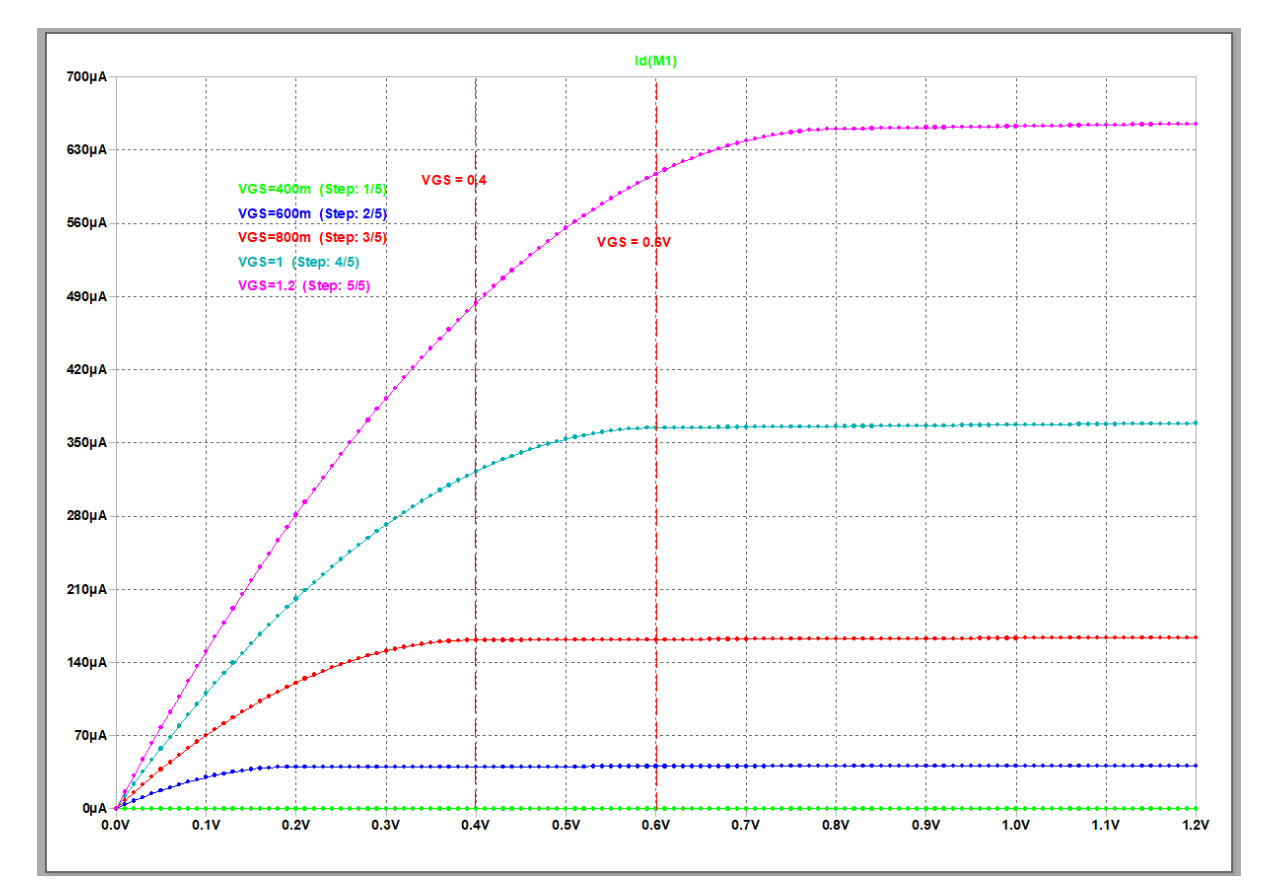
\includegraphics[scale=0.3]{1NMOSImage.png}
    \caption{NMOS I-V Characteristics for various $V_{GS}$ values.}
    \label{fig:nmos_iv_curve}
\end{figure}

The simulation produces five curves corresponding to $VGS = 0.4V, 0.6V, 0.8V, 1.0V, and 1.2V$. 

Each curve exhibits two distinct regions:

\textbf{Linear Region}: For small $VDS$ (where $VDS < VGS - Vth$), the drain current increases approximately linearly with $VDS$. The transistor behaves as a voltage-controlled resistor.
\textbf{Saturation Region:} When $VDS \geq VGS - Vth$, the channel pinches off and $I_D$ becomes nearly independent of $VDS$. The slight upward slope in saturation is due to channel-length modulation ($\lambda = 0.02V^{-1}$).
Verification Calculation $(VGS = 1.2V)$:

Given: $K_P = 200\,\mu\text{A/V}^2$, $W = 10\,\mu\text{m}$, $L = 1\,\mu\text{m}$, $V_{th} = 0.4\,\text{V}$, and $\lambda = 0.02\,\text{V}^{-1}$.

\begin{equation}
\beta = K_P \frac{W}{L}
\end{equation}

\[
\beta = 200\,\mu \times \frac{10}{1} = 2000\,\mu\text{A/V}^2
\]

At saturation with $V_{DS} = 1.2\,\text{V}$, the drain current is

\begin{equation}
I_D = \frac{\beta}{2}(V_{GS} - V_{th})^2(1 + \lambda V_{DS})
\end{equation}

Substituting the values,

\[
I_D = \frac{2000}{2}(1.2 - 0.4)^2(1 + 0.02 \times 1.2)
\]

Evaluating,

\[
I_D = 1000 \times 0.64 \times 1.024 = 655.4\,\mu\text{A}
\]

This closely matches the simulated value, confirming the accuracy of the model.

The effect of channel-length modulation is observed through the parameter $\lambda$. If $\lambda = 0$, the saturation characteristics would be perfectly flat. A non-zero value of $\lambda = 0.02\,\text{V}^{-1}$ introduces a finite output resistance given by

\begin{equation}
r_o = \frac{1}{\lambda I_D}.
\end{equation}

For a drain current of $I_D = 640\,\mu\text{A}$,

\begin{equation}
r_o = \frac{1}{0.02 \times 640 \times 10^{-6}} \approx 78\,\text{k}\Omega.
\end{equation}

This effect is significant in analogue circuit design, as a higher output resistance directly improves amplifier gain.

\subsection{PMOS Sweep and Explanation}

\textbf{Procedure and Theory}
For PMOS, all polarities are reversed relative to NMOS. The source connects to the higher potential, and conduction occurs when $VGS < V_{th}$ (where $V_{th} < 0$).

\begin{center}
\begin{tabular}{|c|c|c|}
\hline
\textbf{Region} & \textbf{Condition (P-channel)} & \textbf{Description} \\
\hline
Cutoff & $V_{GS} > V_{th}$ & OFF (no current) \\
Triode (Linear) & $V_{GS} < V_{th}, \, V_{DS} > V_{GS}-V_{th}$ & Acts as variable resistor \\
Saturation (Active) & $V_{GS} < V_{th}, \, V_{DS} \le V_{GS}-V_{th}$ & Current source (amplifier region) \\
\hline
\end{tabular}
\end{center}

\textbf{Code and Explanation}

\begin{lstlisting}[caption=PMOS Sweep Simulation Code, label=lst:pmos_sweep]
* Task 2: PMOS I-V DC Sweep with Multiple VGS Curves
.param VGSVAL=-1.2

VGS G 0 DC {VGSVAL}                 * Negative gate voltage for PMOS
VDS D 0 DC 0

M1 D G 0 0 PLEVEL1 W=10u L=1u       * PMOS transistor

* Level 1 PMOS model (note negative VTO)
.model PLEVEL1 PMOS LEVEL=1 VTO=-0.4 KP=200u LAMBDA=0.02

* Sweep VDS 0 to -1.2V, VGS from -0.4V to -1.2V
.dc VDS 0 -1.2 -0.01 VGS -0.4 -1.2 -0.2

.plot DC I(M1)
.end
\end{lstlisting}

The netlist mirrors the NMOS structure but with reversed polarities. 
The $.dc$ command sweeps $V_{DS}$ from $0V$ to $-1.2V$ while stepping $V_{GS}$ from $-0.4V$ (threshold) to $-1.2V$ in $-0.2V$ increments. 
The PMOS model uses VTO = $-0.4V$ to reflect the negative threshold voltage.

\textbf{Results and Discussion}

\begin{figure}[H]
    \centering
    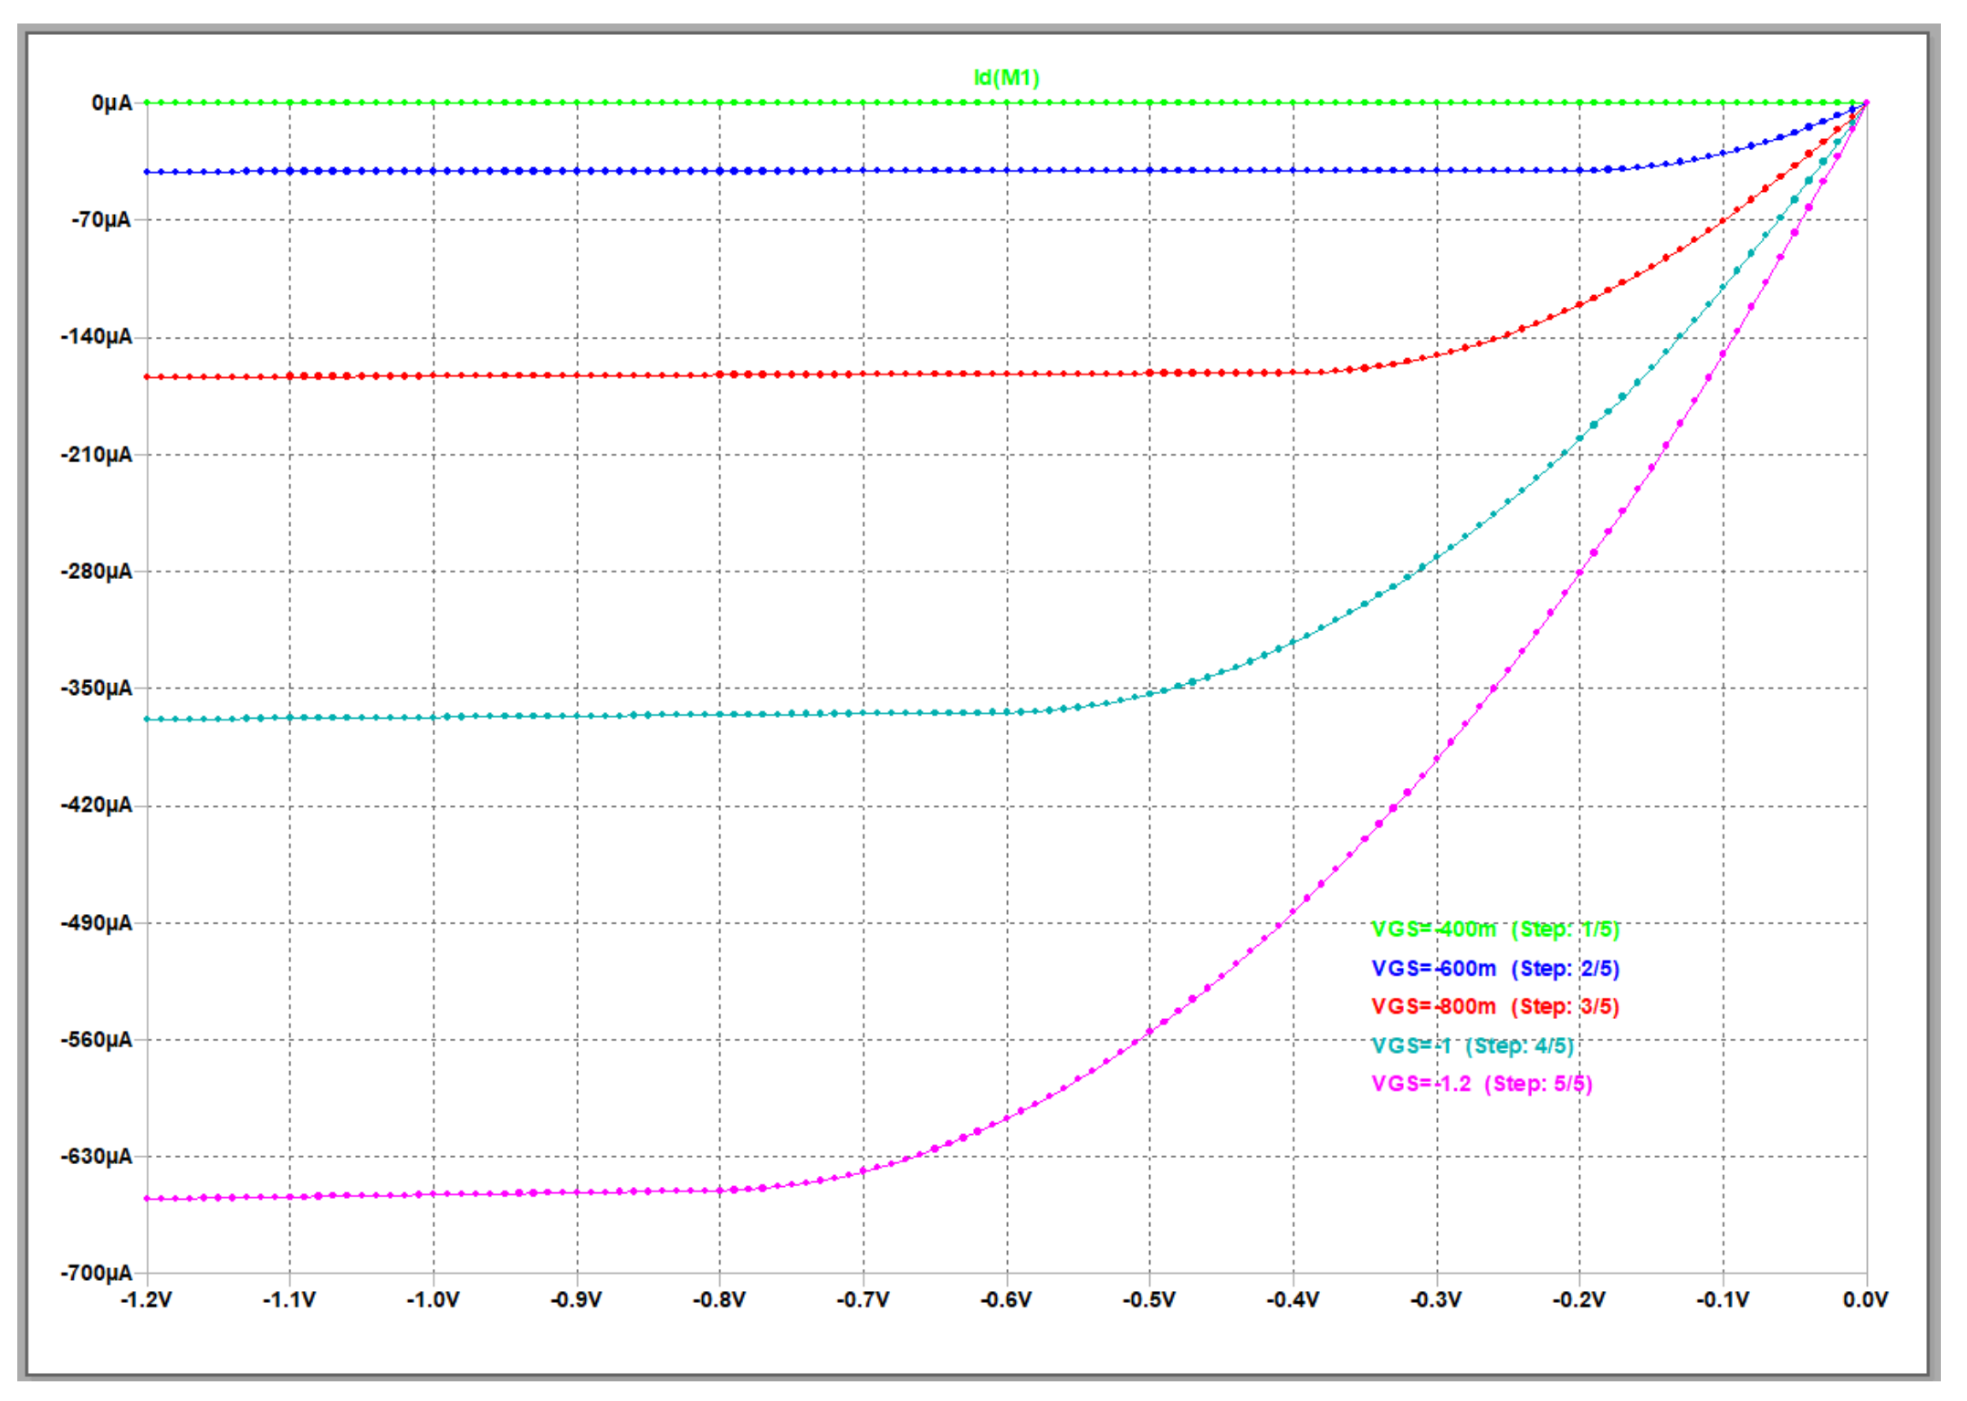
\includegraphics[scale=0.18]{1PMOSImage.png}
    \caption{PMOS I-V Characteristics for various $V_{GS}$ values.}
    \label{fig:pmos_iv_curve}
\end{figure}

From \textbf{Figure \ref{fig:pmos_iv_curve}}, we observe five curves corresponding to 
$VGS = -0.4V, -0.6V, -0.8V, -1.0V,$ and $-1.2V$.

The curves mirror NMOS behaviour but appear in the third quadrant. Key observations are as follows.

In the linear region, the drain current increases steeply for small values of $|V_{DS}|$. In the saturation region, the current reaches a plateau when
\begin{equation}
|V_{DS}| \ge |V_{GS}| - |V_{th}|.
\end{equation}

For verification with $V_{GS} = -1.2\,\text{V}$, the drain current magnitude is

\begin{equation}
I_D = \frac{\beta}{2}(V_{SG} - |V_{th}|)^2
\end{equation}

\[
I_D = \frac{2000}{2}(1.2 - 0.4)^2 = 640\,\mu\text{A}.
\]

The magnitude matches that of the NMOS device because identical $K_P$ and $W/L$ ratios were used. In practical CMOS technologies, PMOS devices typically have a $K_P$ value approximately half that of NMOS due to lower hole mobility. As a result, PMOS transistors are often designed to be approximately twice as wide to achieve matched drive strength.

\subsection{Task 3, Gain Factor Consolidation and Comparison}

\textbf{Procedure and Theory}

This task investigates how transistor geometry affects the drain current through the gain factor $\beta$. From Tasks 1 and 2, the saturation drain current is given by

\begin{equation}
I_D = \frac{\beta}{2}(V_{GS} - V_{th})^2(1 + \lambda V_{DS}).
\end{equation}

The gain factor $\beta$ is defined as

\begin{equation}
\beta = \mu_n C_{ox} \frac{W}{L} = K_P \frac{W}{L}.
\end{equation}

Substituting this expression for $\beta$ into the saturation current equation yields

\begin{equation}
I_D = \frac{K_P}{2} \cdot \frac{W}{L} \cdot (V_{GS} - V_{th})^2(1 + \lambda V_{DS}).
\end{equation}

For fixed values of $V_{GS}$, $V_{DS}$, and $L$, this expression simplifies to

\begin{equation}
I_D = k \cdot W,
\end{equation}

\textbf{Question 1}

From the $.param$ lines:

\[
VGS = 1.2 V
VDS = 1.2 V
L = 1 \mu m
\]

where $k$ is a constant. This result predicts a linear relationship between the drain current $I_D$ and the transistor width $W$, which is verified through simulation.

\textbf{VTO (Threshold Voltage):}
Symbol: $V_T$ or $V_{th}$. Units: Volts (V).

Zero-bias threshold voltage \- the minimum gate-source voltage required to form a conducting inversion channel. Below this voltage, the transistor is in cutoff. Determined by gate material work function, oxide thickness, substrate doping, and interface charges. In our simulation: VTO = 0.4V (NMOS), -0.4V (PMOS).

\textbf{KP (Transconductance Parameter):}
Symbol: $k'$ or $\mu C_{ox}$. Units: A/V$^2$.

Intrinsic transconductance parameter representing the product of carrier mobility ($\mu$) and gate oxide capacitance per unit area ($C_{ox}$):
\begin{equation}
KP = \mu \cdot C_{ox} = \mu \cdot \frac{\varepsilon_{ox}}{t_{ox}}
\end{equation}

Determines current drive capability. The gain factor is $\beta = (W/L) \cdot KP$, so $I_D \propto KP$. NMOS typically has 2-3$\times$ higher KP than PMOS due to higher electron mobility. In our simulation: KP = 200$\mu$A/V$^2$ for both types.

\textbf{LAMBDA (Channel-Length Modulation):}
Symbol: $\lambda$. Units: V$^{-1}$. Default: 0.0.

Channel-length modulation coefficient accounting for effective channel shortening as $V_{DS}$ increases in saturation. Without LAMBDA, saturation curves would be perfectly flat (infinite output resistance). With LAMBDA:
\begin{equation}
I_D(sat) = \frac{\beta}{2}(V_{GS} - V_T)^2(1 + \lambda V_{DS})
\end{equation}

Output resistance: $r_o = 1/(\lambda I_D)$. Inversely proportional to channel length: $\lambda \propto 1/L$. Analogous to inverse Early voltage in BJTs. In our simulation: $\lambda = 0.02$ V$^{-1}$, causing $\sim$2.4\% current increase across 1.2V $V_{DS}$ range.

\textbf{Code and Explanation}

\begin{lstlisting}[caption=PMOS Sweep Simulation Code, label=lst:beta_sweep]
* Task 3: Beta Gain Factor Sweep
.param VGSVAL=1.2 VDSVAL=1.2
.param LVAL=1u

VGS G 0 DC {VGSVAL}
VDS D 0 DC {VDSVAL}

M1 D G 0 0 NLEVEL1 W={WVAL} L={LVAL}

.model NLEVEL1 NMOS LEVEL=1 VTO=0.4 KP=200u LAMBDA=0.02

.step param WVAL 2u 20u 2u          * Sweep W from 2um to 20um
.op                                 * DC operating point analysis

.end
\end{lstlisting}

The \texttt{.step} command varies W while \texttt{.op} calculates the DC operating point for each value. Results appear in the SPICE log rather than as a plot.

\textbf{Question 2B}

The standard textbook equation for saturation current is:
\begin{equation}
I_D = \frac{\beta}{2}(V_{GS} - V_T)^2 \quad \text{where } \beta = \frac{W}{L} \cdot \mu_n C_{ox}
\end{equation}

The complete SPICE Level 1 equation is:
\begin{equation}
I_D = \frac{KP}{2} \cdot \frac{W_{eff}}{L_{eff}} \cdot (V_{GS} - VTO)^2 \cdot (1 + LAMBDA \cdot V_{DS})
\end{equation}

To simplify the SPICE model to match textbook equations, the following assumptions are made:

\textbf{1. LAMBDA = 0 (or very small):}
The term $(1 + \lambda V_{DS})$ is set to 1, neglecting channel-length modulation. This assumes perfectly flat I-V curves in saturation with infinite output resistance. In our simulation, $\lambda = 0.02$ causes only a $\sim$2.4\% variation, which is small but non-zero.

\textbf{2. No body effect ($\gamma = 0$ or $V_{SB} = 0$):}
The body effect modifies threshold voltage as:
\begin{equation}
V_T = V_{T0} + \gamma(\sqrt{|2\phi_F + V_{SB}|} - \sqrt{|2\phi_F|})
\end{equation}
When bulk and source are both at ground ($V_{SB} = 0$), this term vanishes and $V_T = V_{T0}$, which is our case.

\textbf{3. Long-channel approximation:}
Velocity saturation is neglected, assuming drift velocity remains proportional to electric field. Valid for $L \geq 1\mu$m. Short-channel effects (DIBL, threshold roll-off) are ignored.

\textbf{4. No mobility degradation:}
Carrier mobility $\mu$ is assumed constant, independent of $V_{GS}$. In reality, high vertical electric fields reduce mobility, but Level 1 ignores this.

\textbf{5. Ideal effective dimensions:}
$W_{eff} = W$ and $L_{eff} = L$ (no parasitic effects). When $LD = WD = XL = XW = DEL = 0$, drawn and effective dimensions are equal.

\textbf{6. Subthreshold conduction ignored:}
For $V_{GS} < V_T$, Level 1 assumes $I_D = 0$. In reality, exponential subthreshold current exists: $I_D \propto \exp(V_{GS}/nV_t)$.

\textbf{Verification of equivalence:}
If $KP = \mu_n C_{ox}$, then:
\begin{equation}
\beta_{textbook} = \frac{W}{L} \cdot \mu_n C_{ox} = \frac{W}{L} \cdot KP = \beta_{SPICE}
\end{equation}
With $LAMBDA = 0$, $V_{SB} = 0$, and ideal geometry, the equations become identical.

\begin{equation}
I_D = \frac{K_P}{2} \frac{W}{L}(V_{GS} - V_{th})^2,
\end{equation}

with no body-effect corrections included.

\textbf{Results and Discussion}

\begin{lstlisting}[caption=Beta Sweep Simulation Code, label=lst:beta_sweep]
* --- Fixed Bias Parameters ---
.param VGSVAL=1.2
.param VDSVAL=1.2
.param LVAL= 1u

* --- Voltage Sources ---
VGS G 0 DC {VGSVAL}
VDS D 0 DC {VDSVAL}

* --- NMOS with L=2um (doubled) ---
M1 D G 0 0 NLEVEL1 W={WVAL} L={LVAL}

* --- Model ---
.model NLEVEL1 NMOS LEVEL=1 VTO=0.4 KP=200u LAMBDA=0.02

* --- Sweep W ---
.step param WVAL 2u 20u 2u

* --- Analysis ---
.op
.print OP I(M1)

.end
\end{lstlisting}

\begin{figure}[H]
    \centering
    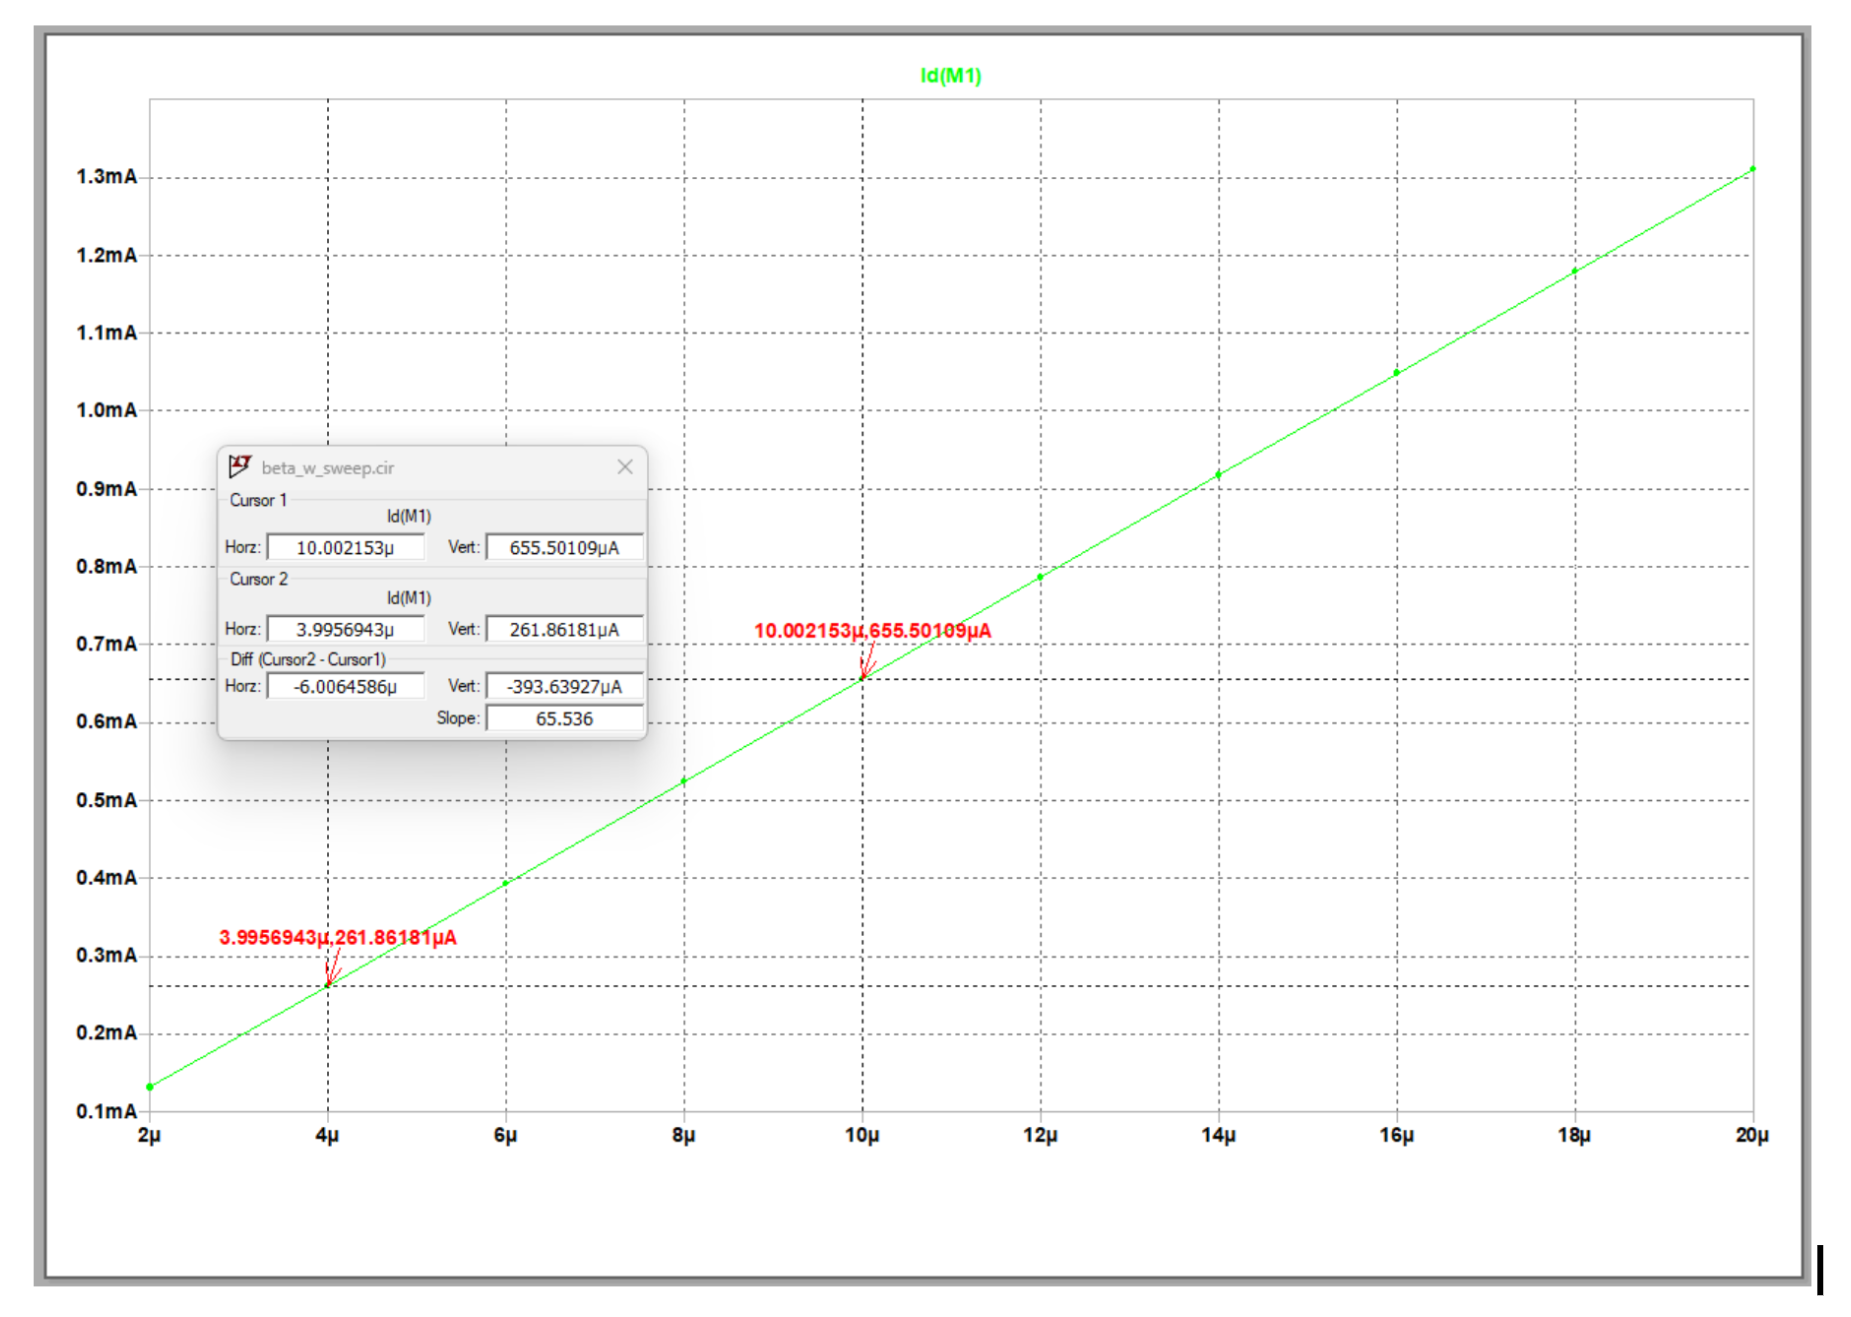
\includegraphics[scale=0.18]{1BetaVerify.png}
    \caption{Beta Sweep}
    \label{fig:beta_iv_curve}
\end{figure}

\textbf{Figure \ref{fig:beta_iv_curve}}, shows the linear relationship between drain current $I_D$ and transistor width $W$. Each data point corresponds to a different width from $2\mu m$ to $20\mu m$.

The theoretical slope can be derived from the saturation drain current expression using the given parameters,

\begin{equation}
I_D = \frac{K_P}{2L}(V_{GS} - V_{th})^2(1 + \lambda V_{DS}) \cdot W.
\end{equation}

Differentiating with respect to the transistor width $W$ gives the slope,

\begin{equation}
\text{Slope} = \frac{dI_D}{dW} = \frac{K_P}{2L}(V_{GS} - V_{th})^2(1 + \lambda V_{DS}).
\end{equation}

Substituting the values $K_P = 200\,\mu\text{A/V}^2$, $L = 1\,\mu\text{m}$, $V_{GS} = 1.2\,\text{V}$, $V_{th} = 0.4\,\text{V}$, $\lambda = 0.02\,\text{V}^{-1}$, and $V_{DS} = 1.2\,\text{V}$,

\begin{equation}
\text{Slope} = \frac{200\,\mu}{2 \times 1\,\mu}(1.2 - 0.4)^2(1 + 0.02 \times 1.2).
\end{equation}

Evaluating,

\begin{equation}
\text{Slope} = 100 \times 0.64 \times 1.024 = 65.54\,\mu\text{A}/\mu\text{m}.
\end{equation}

From simulation, taking two points such as $W = 20\,\mu\text{m}$ with $I_D \approx 1310\,\mu\text{A}$ and $W = 2\,\mu\text{m}$ with $I_D \approx 131\,\mu\text{A}$,

\begin{equation}
\text{Slope} = \frac{1310 - 131}{20 - 2} = \frac{1179}{18} \approx 65.5\,\mu\text{A}/\mu\text{m}.
\end{equation}

This closely matches the theoretical prediction, confirming that $I_D \propto W$.

\textbf{Doubling Channel Length}

If the channel length is doubled to $L = 2\,\mu\text{m}$, then from the definition of the gain factor,

\begin{equation}
\beta = K_P \frac{W}{L}.
\end{equation}

The new gain factor becomes

\begin{equation}
\beta_{\text{new}} = K_P \frac{W}{2L} = \frac{\beta_{\text{original}}}{2}.
\end{equation}

As a result, the drain current $I_D$ is halved for all values of $W$. Consequently, the slope of the $I_D$ versus $W$ characteristic becomes

\begin{equation}
\text{New Slope} = \frac{65.54}{2} = 32.77\,\mu\text{A}/\mu\text{m}.
\end{equation}

This result illustrates why shorter channel lengths are preferred in transistor design to achieve higher drive current.

\textbf{Results and Discussion}

\begin{figure}[H]
    \centering
    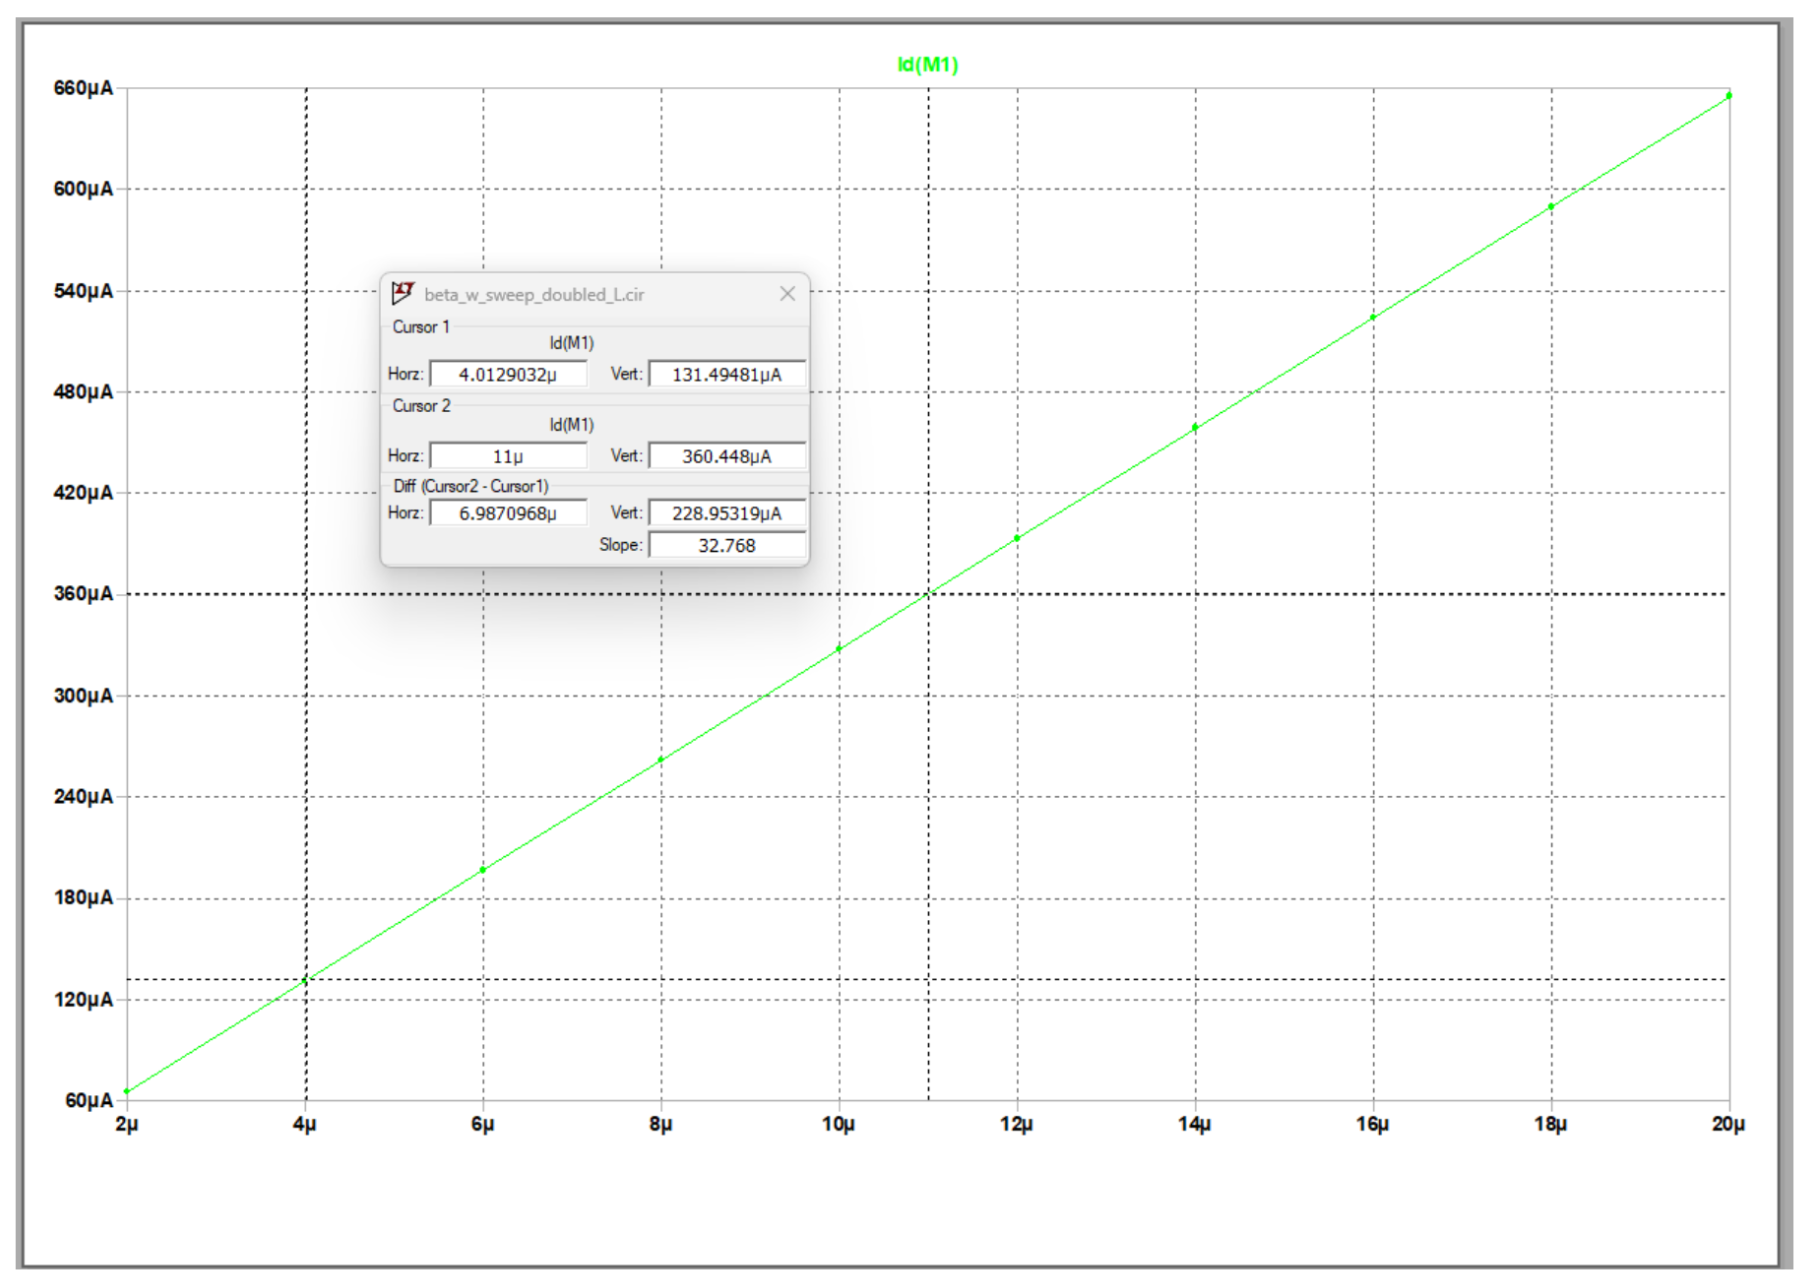
\includegraphics[scale=0.18]{1BetaDoubledL.png}
    \caption{PMOS I-V Characteristics for various $V_{GS}$ values.}
    \label{fig:beta_2x_curve}
\end{figure}

\textbf{Figure \ref{fig:beta_2x_curve}} shows the linear relationship between drain current $I_D$ and transistor width $W$ when the channel length is doubled to $L = 2\,\mu\text{m}$. Each data point corresponds to a different width from $2\mu m$ to $20\mu m$.

\textbf{Reducing VGS}

When $V_{GS} < V_{th}$, for example $V_{GS} = 0.3\,\text{V} < 0.4\,\text{V}$, the transistor operates in the cutoff region. In this condition, no inversion layer is formed and the drain current satisfies

\begin{equation}
I_D \approx 0,
\end{equation}

independent of the transistor width $W$. This behaviour explains why the threshold voltage defines the effective on/off boundary in digital switching applications.

\textbf{Why PMOS is wider than NMOS}

In Task 2, equal values of $K_P$ were used for NMOS and PMOS devices. In practice, however, the process transconductance parameters differ:

\begin{equation}
K_{P,n} = \mu_n C_{ox} \approx 200\,\mu\text{A/V}^2,
\end{equation}

\begin{equation}
K_{P,p} = \mu_p C_{ox} \approx 80\text{--}100\,\mu\text{A/V}^2.
\end{equation}

Since the hole mobility is lower than the electron mobility, with $\mu_p \approx 0.4\mu_n$, a PMOS transistor must be approximately $2$--$2.5$ times wider than an NMOS transistor to achieve symmetric rise and fall times in a CMOS inverter.

\textbf{Task 4, Iterative Solutions}

SPICE solves circuits containing nonlinear devices, such as diodes and transistors, using iterative numerical methods. Unlike linear circuits, where Kirchhoff’s laws lead to direct algebraic solutions, nonlinear device equations require iterative root-finding techniques.

Applying Kirchhoff’s Voltage Law (KVL) to the series circuit gives

\begin{equation}
V_s - I R - V_d = 0.
\end{equation}

The diode current is described by the Shockley equation,

\begin{equation}
I = I_s \left( e^{V_d / n V_t} - 1 \right).
\end{equation}

Substituting this expression for $I$ into the KVL equation yields

\begin{equation}
f(V_d) = V_s - R I_s \left( e^{V_d / n V_t} - 1 \right) - V_d = 0.
\end{equation}

This is a nonlinear equation in $V_d$ and cannot be solved analytically.

To find the root of $f(V_d) = 0$, SPICE employs the Newton--Raphson method, which iterates according to

\begin{equation}
V_d^{(k+1)} = V_d^{(k)} - \frac{f\!\left(V_d^{(k)}\right)}{f'\!\left(V_d^{(k)}\right)}.
\end{equation}

The derivative of $f(V_d)$ is

\begin{equation}
f'(V_d) = -\frac{R I_s}{n V_t} e^{V_d / n V_t} - 1.
\end{equation}

Convergence is achieved when the change in voltage satisfies $|\Delta V_d| < \varepsilon$, where $\varepsilon$ is a chosen tolerance.

In earlier tasks, the Level~1 MOSFET model was used, which also involves nonlinear equations such as

\begin{equation}
I_D = \frac{\beta}{2}(V_{GS} - V_{th})^2.
\end{equation}

When SPICE computes the DC operating point, it applies the Newton\-Raphson method internally to solve these nonlinear device equations simultaneously with the Kirchhoff current and voltage constraints.

\begin{table}[h]
\centering
\begin{tabular}{ll}
\hline
\textbf{Parameter} & \textbf{Value} \\
\hline
$V_s$   & $5\,\text{V}$ \\
$R$     & $1\,\text{k}\Omega$ \\
$I_s$   & $10^{-12}\,\text{A}$ \\
$n$     & $1$ \\
$V_t$   & $26\,\text{mV}$ (at $T = 300\,\text{K}$) \\
\hline
\end{tabular}
\caption{Circuit and diode parameters used in the analysis}
\end{table}

Due to the length of the code, use the link to view the Python script here: (INSERT PYTHON CODE LINK GITHUB HERE).

\textbf{Figure \ref{fig:NRIOutput}} shows the terminal output from running the Newton\-Raphson iterative solver for the diode circuit. The iterations converge to a diode voltage of approximately $0.58\,\text{V}$, yielding a current of about $4.4\,\text{mA}$.

\begin{figure}[H]
    \centering
    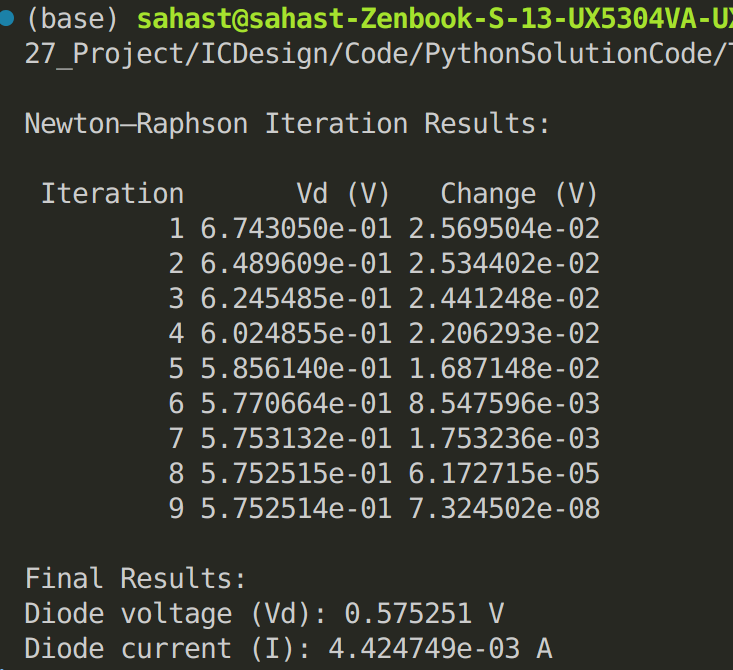
\includegraphics[scale=0.36]{Task4NRI.png}
    \caption{Newton Raphson Terminal Output}
    \label{fig:NRIOutput}
\end{figure}

A cobweb diagram can be used to visualise the convergence of the Newton\-Raphson iterations. \textbf{Figure \ref{fig:newton_cobweb_diagram}} illustrates how successive approximations approach the root of the nonlinear equation.

\begin{figure}[H]
    \centering
    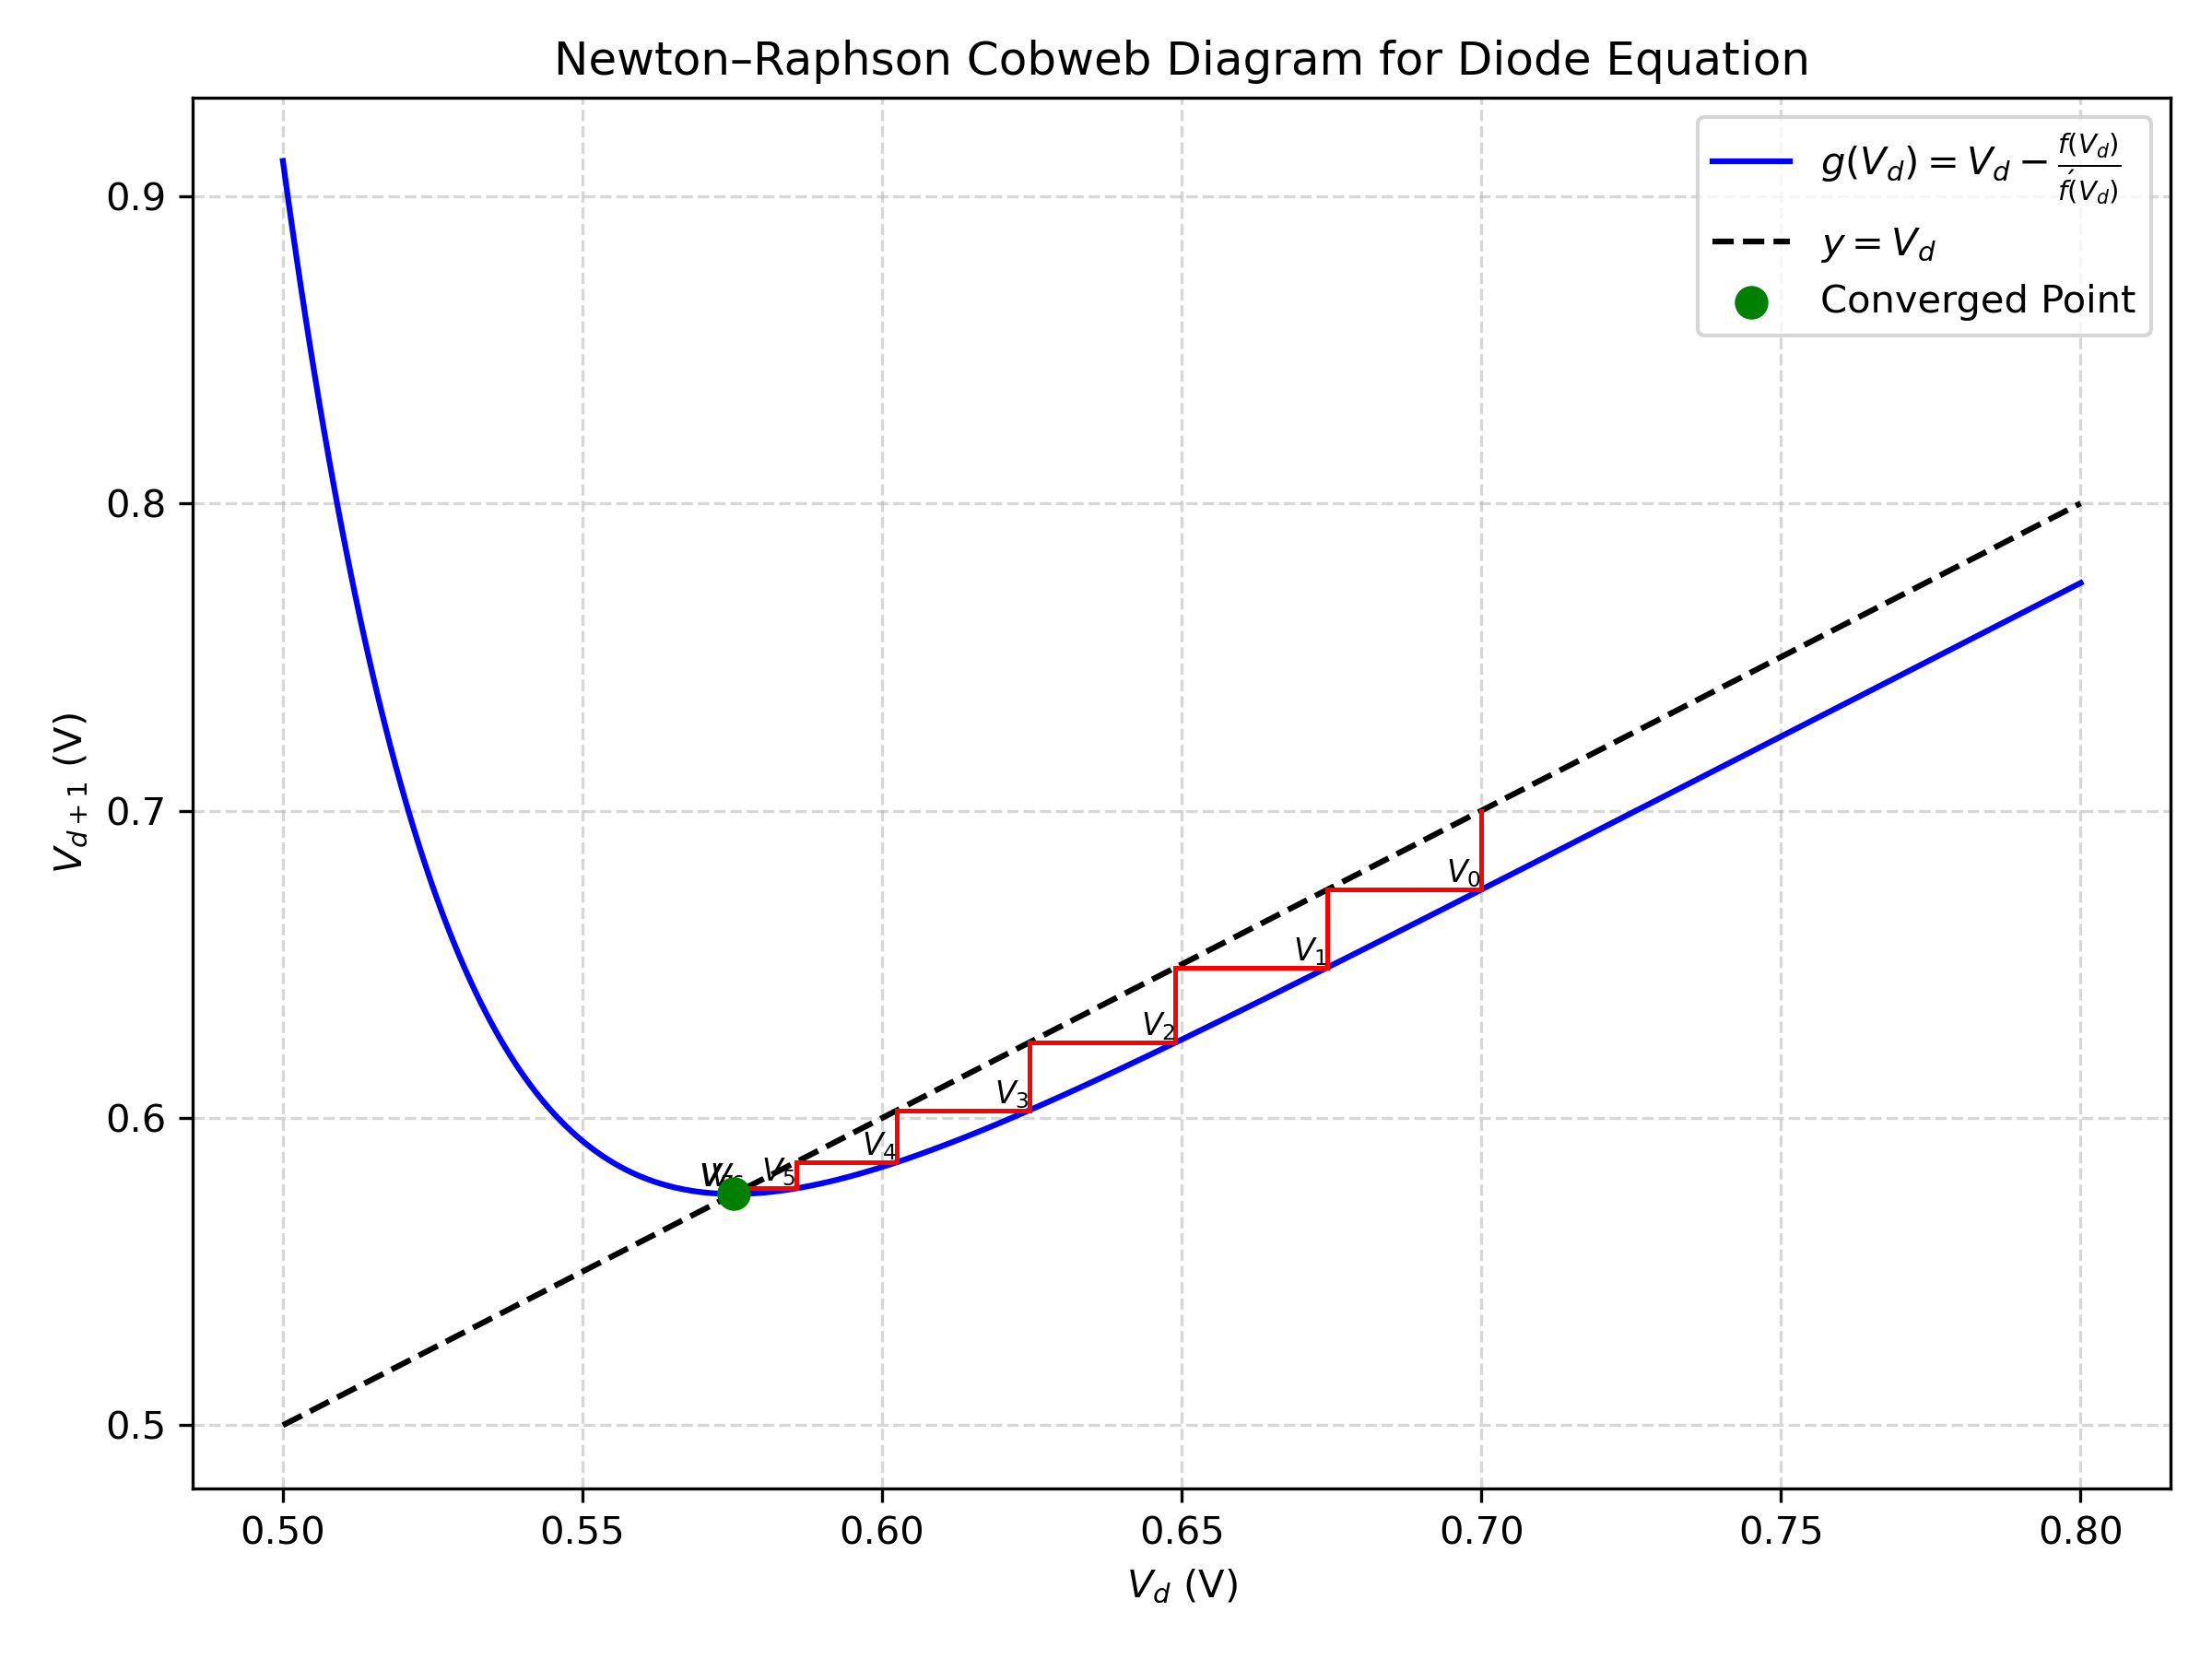
\includegraphics[scale=0.48]{newton_cobweb_diagram.png}
    \caption{Cobweb Diagram Showing the Convergence of Newton\-Raphson Iterations.}
    \label{fig:newton_cobweb_diagram}
\end{figure}

\textbf{Results and Discussion}

The Newton--Raphson method converges rapidly due to its quadratic convergence property, meaning that the number of correct digits approximately doubles with each iteration. From the numerical output, six-digit accuracy is achieved in approximately seven iterations. This computational efficiency is the reason SPICE employs the Newton--Raphson algorithm for DC operating-point analysis.

Verification of the solution can be performed using Kirchhoff’s Voltage Law,

\begin{equation}
V_s - I R - V_d = 5 - (4.383 \times 10^{-3})(1000) - 0.6166 = 0,
\end{equation}

which confirms that the computed values satisfy the circuit constraints.

When SPICE analyses the MOSFET circuits from Tasks~1--3, it formulates nonlinear equations from the device models, such as $I_D = f(V_{GS}, V_{DS})$, and combines them with the Kirchhoff voltage and current constraints. 

These equations are linearised through construction of the Jacobian matrix, which is the multivariable generalisation of the derivative $f'(x)$. 

SPICE then iterates using the Newton\-Raphson method until all node voltages converge.

The \texttt{.OPTIONS} command in SPICE controls convergence parameters such as \texttt{RELTOL} (relative tolerance) and \texttt{ITL1} (DC iteration limit), which are directly analogous to the tolerance $\varepsilon$ used in the Python-based implementation.

\subsection{Lab 2}

\textbf{Lab 2: CMOS Inverter Design and Analysis}

\begin{figure}[H]
    \centering
    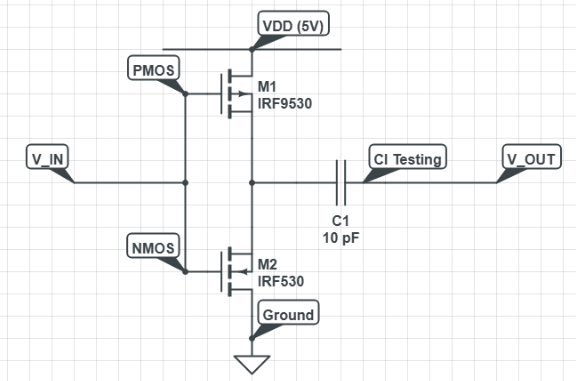
\includegraphics[scale=0.78]{NewCircuit.png}
    \caption{Cobweb Diagram Showing the Convergence of Newton\-Raphson Iterations.}
    \label{fig:CobwebDiagram}
\end{figure}

PMOS (pull-up network)  $20\,\mu\text{m}$, $1\,\mu\text{m}$ \\
NMOS (pull-down network) $10\,\mu\text{m}$, $1\,\mu\text{m}$ \\
added here as it would not be clear in the image.

\textbf{SPICE Template Completion}

The SPICE netlist defines the circuit topology, device models, and analysis type. For DC analysis, we sweep Vin from 0V to 5V to observe the transfer characteristic.

The netlist code is as follows:

\begin{lstlisting}[caption=SPICE template completion, label=lst:SPICE_complete]
* Power supply: 5V DC connected between Vdd node and ground
VDD Vdd 0 DC 5

* Input voltage source: swept from 0 to 5V for DC analysis
Vin in 0 DC 0

* NMOS transistor M1 (pull-down network)
* Terminals: Drain=out, Gate=in, Source=0, Bulk=0
M1 out in 0 0 NMOSLEVEL1 W=10u L=1u

* PMOS transistor M2 (pull-up network)
* Terminals: Drain=out, Gate=in, Source=Vdd, Bulk=Vdd
M2 out in Vdd Vdd PMOSLEVEL1 W=20u L=1u

* DC sweep: Vin from 0V to 5V in 10mV steps
.dc Vin 0 5 0.01

* Plot input and output voltages
.plot DC V(in) V(out)

* NMOS Level 1 model: Vth=0.4V, KP=200uA/V^2, lambda=0.02
.model NMOSLEVEL1 NMOS LEVEL=1 VTO=0.4 KP=200u LAMBDA=0.02

* PMOS Level 1 model: Vth=-0.4V, KP=80uA/V^2, lambda=0.02
.model PMOSLEVEL1 PMOS LEVEL=1 VTO=-0.4 KP=80u LAMBDA=0.02

.end
\end{lstlisting}

The netlist defines complementary NMOS and PMOS transistors that share a common gate (input) and a common drain (output). The PMOS device is sized with a width of $W = 20\,\mu\text{m}$, which is twice that of the NMOS transistor, to compensate for the lower hole mobility. This sizing choice ensures approximately symmetric rise and fall times during switching.

\textbf{1C: DC Transfer Curve}

The DC transfer curve shows the static relationship between input and output. Five operating regions exist based on which transistor is in cutoff, linear, or saturation.

At point A, with $V_{\text{in}} = 0\,\text{V}$, the NMOS transistor has $V_{GS} = 0 < V_{th}$ and is therefore turned off. The PMOS transistor has $V_{SG} = 5\,\text{V} > |V_{th}|$, conducts strongly, and pulls the output voltage such that $V_{\text{out}} \approx V_{DD}$.

At point C, with $V_{\text{in}} = 2.5\,\text{V}$, both transistors operate in saturation. This corresponds to the high-gain transition region, where small changes in the input voltage produce large swings in the output voltage.

At point E, with $V_{\text{in}} = 5\,\text{V}$, the PMOS transistor has $V_{SG} = 0 < |V_{th}|$ and is therefore turned off. The NMOS transistor conducts, pulling the output voltage such that $V_{\text{out}} \approx 0\,\text{V}$.

\begin{table}[h]
\centering
\begin{tabular}{ccccc}
\hline
\textbf{Point} & \textbf{$V_{\text{in}}$ (V)} & \textbf{$V_{\text{out}}$ (V)} & \textbf{NMOS Mode} & \textbf{PMOS Mode} \\
\hline
A & 0   & $\sim 5$   & Cutoff      & Linear      \\
B & 1   & $\sim 5$   & Saturation  & Linear      \\
C & 2.5 & $\sim 2.5$ & Saturation  & Saturation  \\
D & 4   & $\sim 0$   & Linear      & Saturation  \\
E & 5   & $\sim 0$   & Linear      & Cutoff      \\
\hline
\end{tabular}
\caption{Operating regions of NMOS and PMOS transistors at key points on the CMOS inverter voltage transfer characteristic}
\end{table}

The transfer curve can be seen clearly below:

\begin{figure}[H]
    \centering
    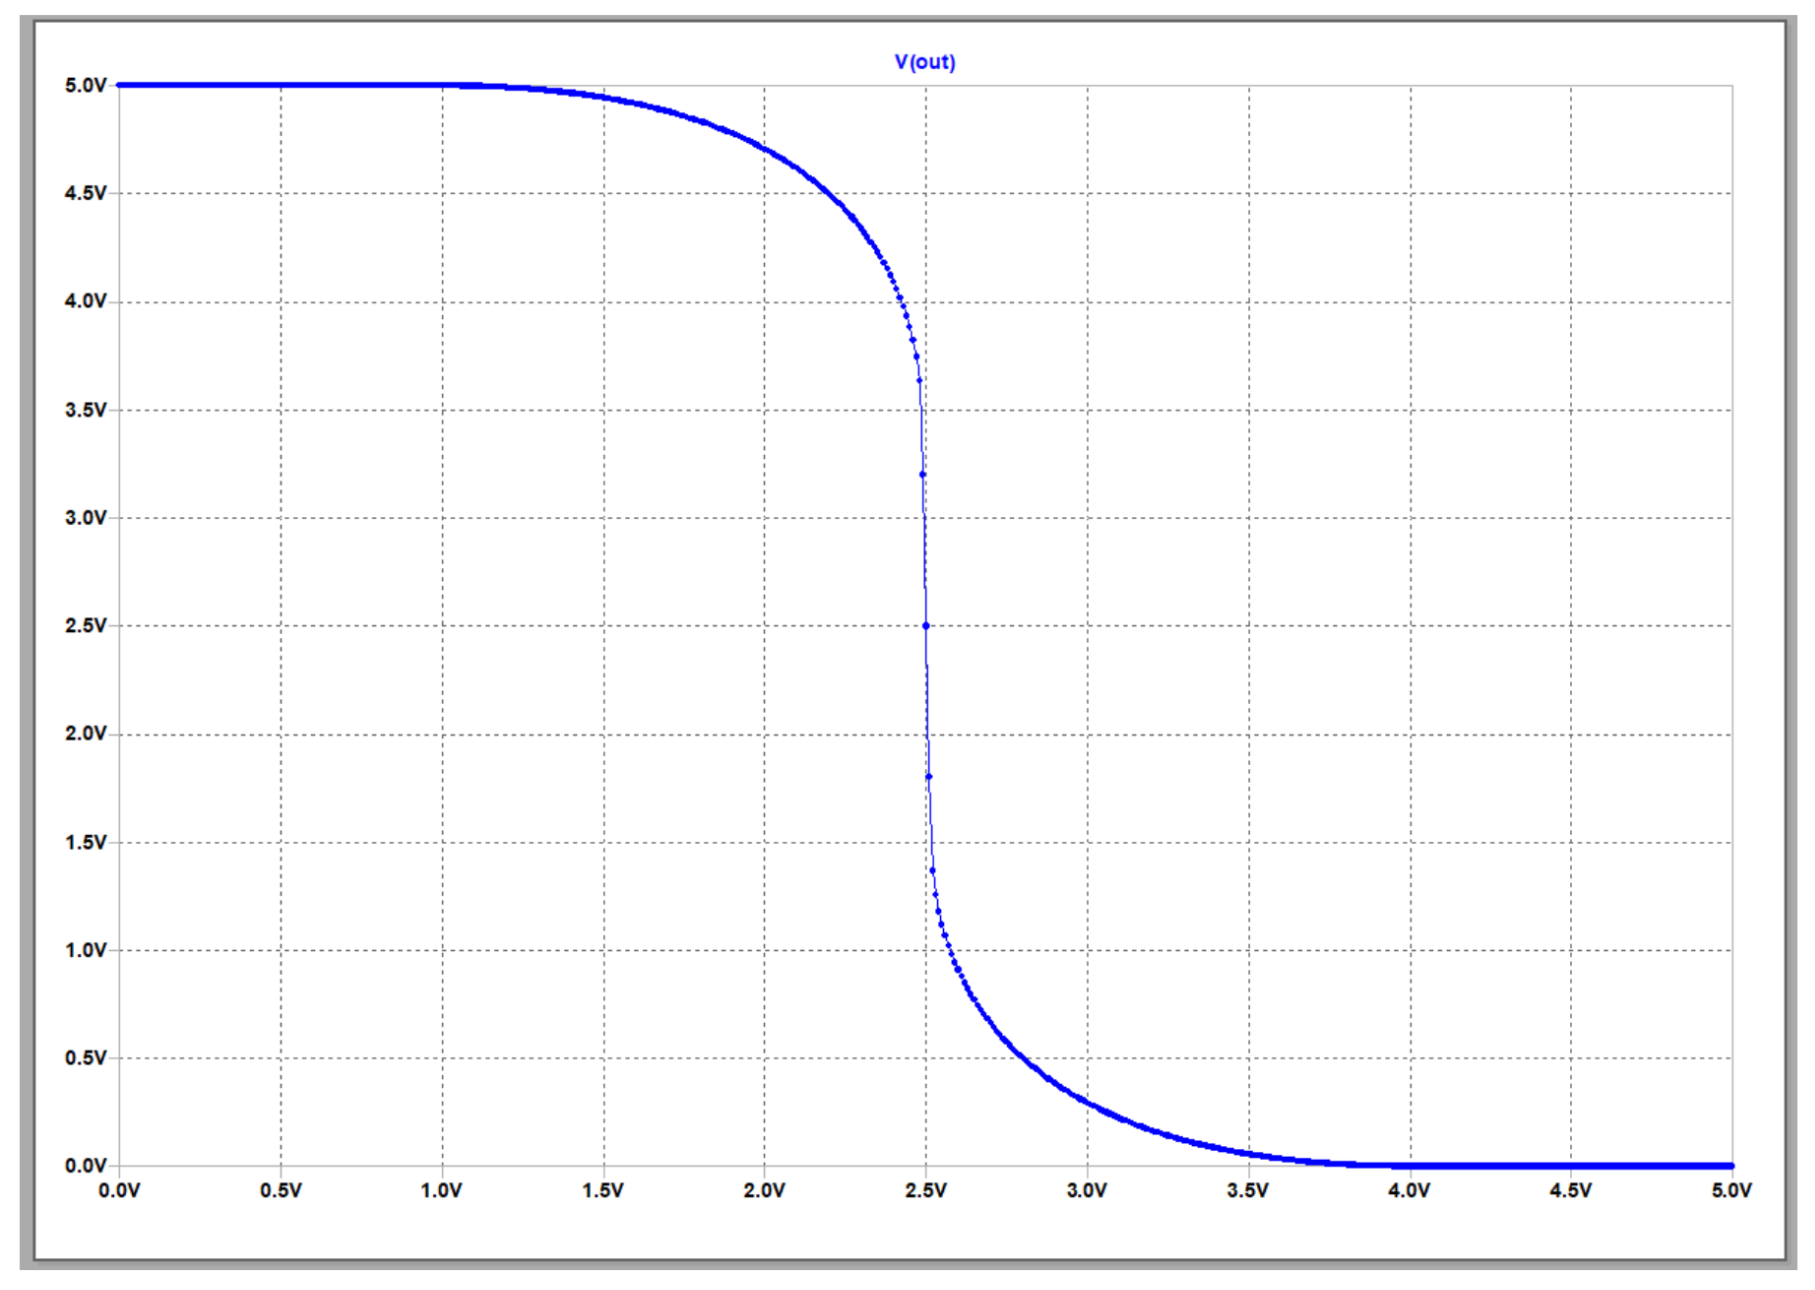
\includegraphics[scale=0.24]{2CMOSInverter.png}
    \caption{CMOS Transfer Curve}
    \label{fig:CMOSTransfer}
\end{figure}

The following figures show the cursor positions for points A through E on the voltage transfer curve.

\begin{figure}[H]
    \centering
    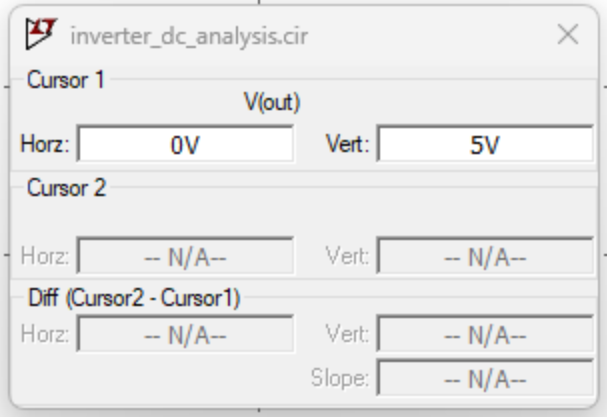
\includegraphics[scale=0.37]{Point1.png}
    \caption{CMOS Point A}
    \label{fig:PointA}
\end{figure}

\begin{figure}[H]
    \centering
    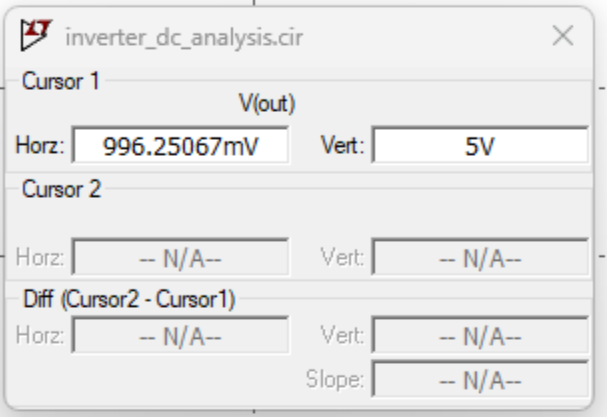
\includegraphics[scale=0.37]{Point2.png}
    \caption{CMOS Point B}
    \label{fig:PointB}
\end{figure}

\begin{figure}[H]
    \centering
    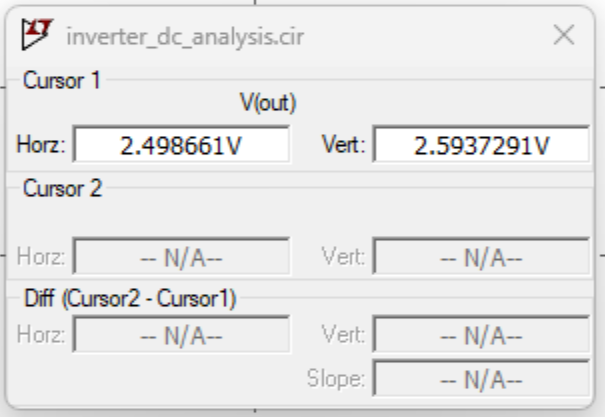
\includegraphics[scale=0.37]{Point3.png}
    \caption{CMOS Point C}
    \label{fig:PointC}
\end{figure}

\begin{figure}[H]
    \centering
    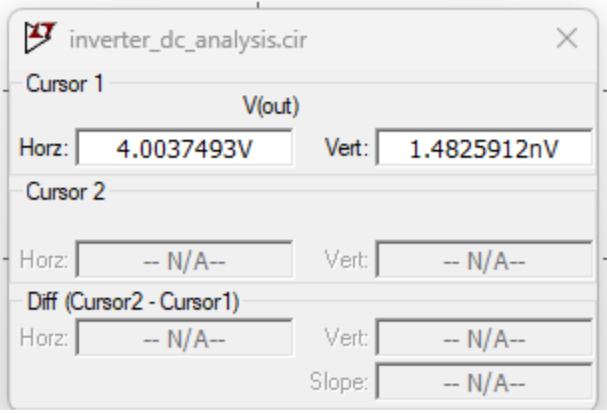
\includegraphics[scale=0.37]{Point4.png}
    \caption{CMOS Point D}
    \label{fig:PointD}
\end{figure}

\begin{figure}[H]
    \centering
    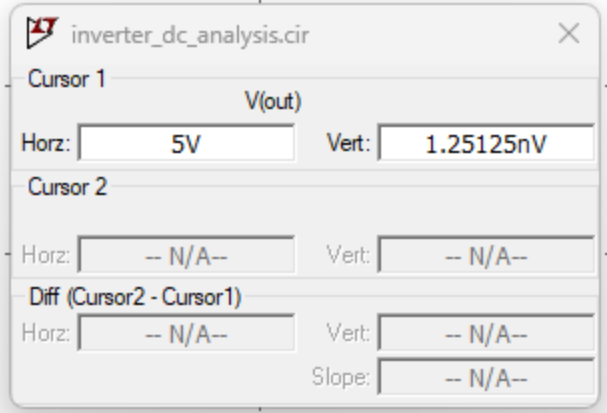
\includegraphics[scale=0.37]{Point5.png}
    \caption{CMOS Point E}
    \label{fig:PointE}
\end{figure}

\textbf{1D NMOS Pull Up Exploration}

By altering the CMOS structure to only use NMOS transistors for both pull-up and pull-down networks, we can observe the impact on the voltage transfer characteristic.
The modified netlist is as follows:

\begin{lstlisting}[caption=NMOS Pull Down, label=lst:pulldown]
* NMOS-only Inverter (Pseudo-NMOS)
VDD Vdd 0 DC 5
Vin in 0 DC 0

* Pull-down NMOS
M1 out in 0 0 NMOSLEVEL1 W=10u L=1u

* Pull-up NMOS (gate tied to VDD - always trying to conduct)
M2 out Vdd Vdd 0 NMOSLEVEL1 W=20u L=1u

.dc Vin 0 5 0.01
.plot DC V(out)
.model NMOSLEVEL1 NMOS LEVEL=1 VTO=0.4 KP=200u LAMBDA=0.02
.end
\end{lstlisting}

\begin{figure}[H]
    \centering
    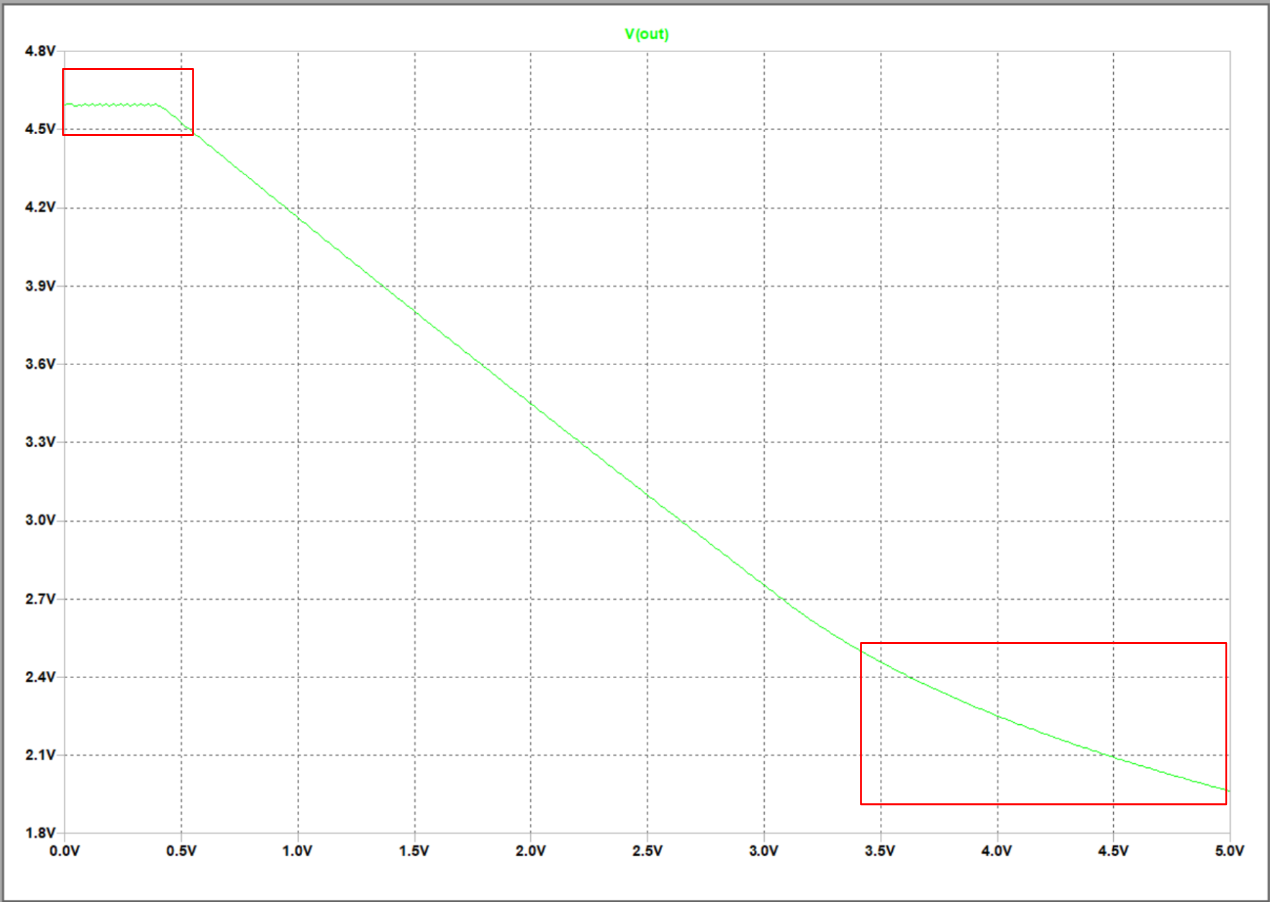
\includegraphics[scale=0.25]{HighlightedNMOSOnly.png}
    \caption{NMOS Pull Down Transfer Curve}
    \label{fig:NMOSOnlyTransfer}
\end{figure}

\textbf{Q1: What is the highest output voltage? Why not 5V?}

The maximum $Vout \approx 4.6V$ ($= VDD - Vth = 5 - 0.4V$). The NMOS pull-up cannot pass a voltage higher than $VGS - Vth$. When Vout approaches $VDD - Vth$, the pull-up NMOS enters cutoff because $VGS = VDD - Vout$ drops below Vth.

\textbf{Q2: What happens to the NMOS pull-up when Vin = 0?}

When $Vin = 0V$, the pull-down M1 is OFF. The pull-up M2 tries to charge the output, but it's operating as a source follower with $VGS = VDD - Vout$. As Vout rises, VGS decreases until $VGS = Vth$, at which point M2 enters cutoff and charging stops.

\textbf{Q3: What happens if this drives another CMOS gate?}

The degraded logic '1' ($4.6V$ instead of $5V$) may not fully turn OFF the PMOS in the next stage. This causes:

\begin{itemize}
  \item Static power dissipation (both transistors partially ON)
  \item Reduced noise margin
  \item Slower switching in subsequent stages
\end{itemize}

\textbf{Q4: Why does PMOS avoid this issue?}

PMOS passes strong '1's because its source connects to VDD. When pulling up, $VSG = VDD - Vout$ remains high until $Vout = VDD$. PMOS can fully charge the output to VDD without the threshold voltage drop limitation.

From the figure above, the appropriate regions have been labelled.

\textbf{Task 2: Inverter Transient Analysis}

Transient analysis characterises the dynamic switching behaviour of the circuit. The key timing parameters are defined as follows.

\begin{equation}
t_{\text{rise}} = t_{90\%} - t_{10\%},
\end{equation}

\begin{equation}
t_{\text{fall}} = t_{10\%} - t_{90\%},
\end{equation}

\begin{equation}
t_{PHL} = t_{\text{out},50\%} - t_{\text{in},50\%} \quad \text{(output falling)},
\end{equation}

\begin{equation}
t_{PLH} = t_{\text{out},50\%} - t_{\text{in},50\%} \quad \text{(output rising)}.
\end{equation}

The design specifications are:

\[
t_{\text{rise}} \le 15\,\text{ns},
\]

\[
t_{\text{fall}} \le 10\,\text{ns},
\]

\[
|t_{PLH} - t_{PHL}| \le 2\,\text{ns}.
\]

\textbf{Code and Explanation}

\begin{lstlisting}[caption=NMOS Pull Down, label=lst:pulldown]
* CMOS Inverter Transient - Original Design
VDD Vdd 0 DC 5
Vin in 0 PULSE(0 5 0ns 5ns 5ns 50ns 100ns)  * 100ns period pulse

M1 out in 0 0 NMOSLEVEL1 W=10u L=1u
M2 out in Vdd Vdd PMOSLEVEL1 W=20u L=1u
CL out 0 10p                                 * 10pF load

.tran 0.1ns 200ns

.model NMOSLEVEL1 NMOS LEVEL=1 VTO=0.4 KP=200u LAMBDA=0.02
.model PMOSLEVEL1 PMOS LEVEL=1 VTO=-0.4 KP=80u LAMBDA=0.02

* Automated measurements
.meas tran t_rise TRIG V(out) VAL=0.5 RISE=1 TARG V(out) VAL=4.5 RISE=1
.meas tran t_fall TRIG V(out) VAL=4.5 FALL=1 TARG V(out) VAL=0.5 FALL=1
.meas tran tPHL TRIG V(in) VAL=2.5 RISE=1 TARG V(out) VAL=2.5 FALL=1
.meas tran tPLH TRIG V(in) VAL=2.5 FALL=1 TARG V(out) VAL=2.5 RISE=1
.meas tran t_skew PARAM='abs(tPHL-tPLH)'
.end
\end{lstlisting}

The \texttt{PULSE} source generates a $0-5V$ square wave with $5ns$ rise/fall times and $100ns$ period. The \texttt{.meas} commands automatically extract timing parameters.

\begin{figure}[H]
    \centering
    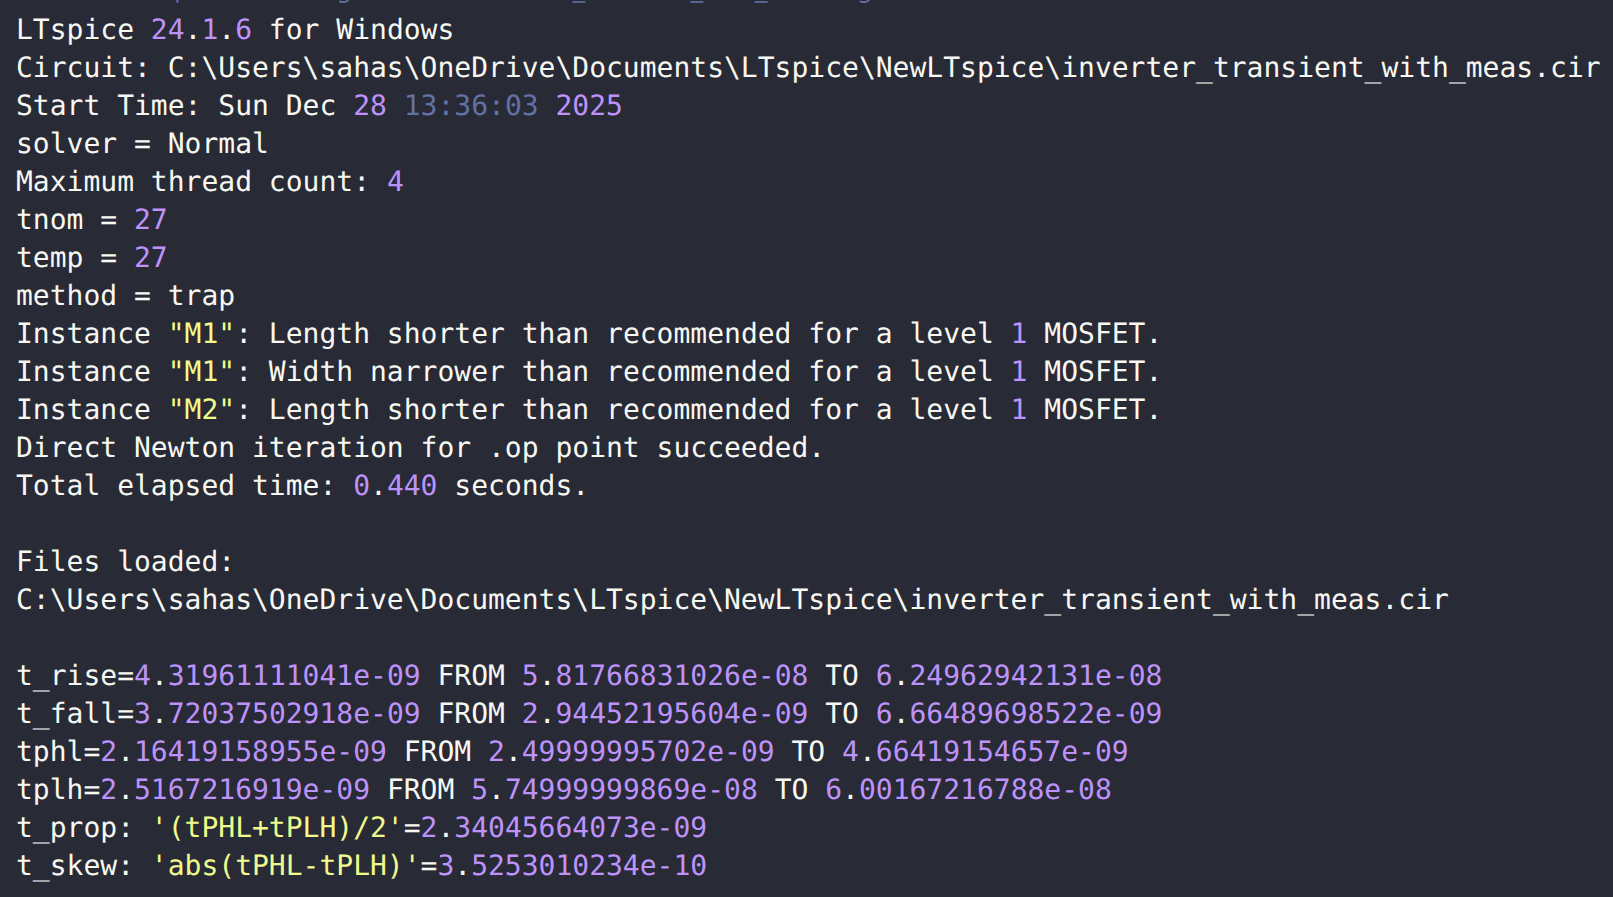
\includegraphics[scale=0.25]{OGTransientAnalysisLog.png}
    \caption{Original Transient Analysis Log Output}
    \label{fig:OGTransientAnalysisLog}
\end{figure}

\section{FPGA Design Labs \- (Labs 4, 5 \& 6)}

\section{Asynchronous Circuit Modelling with Workcraft \- (Labs 7 \& 8)}

\subsection{Lab 7 - C-Element Modelling and Design}

\textbf{Part 1, Theory and Procedure}

The C-element is one of the most fundamental building blocks in asynchronous circuit design. Unlike combinational gates where outputs are purely a function of current inputs, the C-element is a state-holding element with memory. 

Its behaviour is defined as follows: the output transitions HIGH ($Q^+$) only when all inputs are HIGH, the output transitions LOW ($Q^-$) only when all inputs are LOW, and when the inputs have different values, the output retains its previous value. This makes it a synchronisation element that waits for all inputs to agree before changing state.

The state-dependent truth table for a two-input C-element is given by:
\[
\begin{array}{c c c c}
A & B & Q(t) & Q(t+1) \\
\hline
0 & 0 & 0 & 0 \\
0 & 0 & 1 & 0 \\
1 & 1 & 0 & 1 \\
1 & 1 & 1 & 1 \\
0 & 1 & 0 & 0 \\
0 & 1 & 1 & 1 \\
1 & 0 & 0 & 0 \\
1 & 0 & 1 & 1
\end{array}
\]

Signal Transition Graphs (STGs) are an extension of Petri nets specifically designed for specifying asynchronous circuits. 

Each signal event (rising transition denoted '+' or falling transition denoted '-') becomes a Petri net transition. 

Places between transitions hold tokens representing the current state, and arcs define causality - which events must occur before others can fire.

\textbf{part 1, C-Element STG construction}



\textbf{Part 1, Results and Discussion}

The structure enforces AND-causality by requiring both $in1^+$ and $in2^+$ to fire before $out^+$ is enabled. 

In Petri net terms, $out^+$ has two input places that must both contain tokens. The implicit places represent waiting states; for example, after $in1^+$ fires, the system waits for $in2^+$ before allowing $out^+$ to occur. 

The initial marking, with tokens on the arcs from $out^-$ to the input rising transitions, represents the starting condition where all signals are LOW and the system is ready for a new SET phase. 

The STG allows concurrency, so $in1^+$ and $in2^+$ may occur in any order, reflecting that their relative timing is actually unimportant.

This can be seen in the STG diagram below:

\begin{large}
    IMAGE SHOWING STG OF C-ELEMENT HERE
\end{large}

The trace corresponding to the STG is shown here, with two runs of the C-element behaviour:

\begin{large}
 IMAGE SHOWING THE TRACE OF THE C-ELEMENT HERE.
\end{large}

 . Circuit timing diagram generated from the trace is shown below:

\begin{large}
    IMAGE SHOWING THE TIMING DIAGRAM OF THE C-ELEMENT HERE.
\end{large}

\textbf{Part 2, Simulation and Verification}

\textbf{Part 2, Procedure and theory}

Before synthesising an STG into a circuit, it must be verified against key correctness properties. 

Consistency requires every signal to alternate strictly between rising and falling transitions, meaning $in1^+ \rightarrow in1^-$ must occur before another $in1^+$, ensuring valid digital behaviour. 

Deadlock-freeness guarantees progress by requiring that from every reachable state, at least one transition is enabled, so the system never reaches a state where no action is possible. 

Input-properness ensures that input transitions are controlled only by the environment and are never disabled by internal circuit behaviour. Output-persistence requires that once an output or internal transition becomes enabled, it cannot be disabled by another firing transition, which is essential for hazard-free operation.

Verification is performed by first activating the Simulation tool [M] and manually firing enabled transitions, or by pasting a trace such as $in2^+ \rightarrow in1^+ \rightarrow out^+ \rightarrow in1^- \rightarrow in2^- \rightarrow out^-$. 

After simulating a trace, a timing diagram can be generated using the \textit{Generate trace diagram} option. 

Formal verification is then carried out via \textit{Verification} $\rightarrow$ \textit{Consistency (MPSat)}, followed by deadlock freeness, input properness, and output persistency checks, or by using the combined option \textit{Conformation, deadlock freeness, and output persistency (reuse unfolding)}.

\textbf{Part 2, Results and Discussion}

Consistency holds because the STG enforces strict alternation of transitions, with each signal following a cyclic pattern $+ \rightarrow - \rightarrow + \rightarrow -$. 

Deadlock-freeness is satisfied since at least one transition is always enabled: initially $in1^+$ and $in2^+$ are enabled, after they fire $out^+$ becomes enabled, and the cycle repeats indefinitely. 

Input-properness holds because input transitions ($in1^\pm$, $in2^\pm$) are controlled solely by the environment and are not disabled by output behaviour. 

Output-persistence is satisfied because once $out^+$ or $out^-$ becomes enabled, it cannot be disabled by any input transition; for example, after $in1^+$ and $in2^+$ fire, $out^+$ is guaranteed to occur since no input can remove the required tokens.

Verification results from Workcraft are shown below:

\begin{large}
    IMAGE SHOWING THE VERIFICATION RESULTS FOR C-ELEMENT HERE.
\end{large}

\textbf{Part 3, Synthesis - Complex Gate vs Technology Mapping}

\textbf{Part 3, Procedure and Theory}

Asynchronous circuit synthesis converts an STG specification into a gate-level implementation. Workcraft supports two main approaches. In complex-gate synthesis, a single Boolean equation is derived for each output or internal signal. For the C-element this gives
\[
out = (out \lor in2)\land in1 \;\lor\; in2 \land out,
\]
which simplifies to
\[
out = (in1 \land in2) \;\lor\; (in1 \land out) \;\lor\; (in2 \land out).
\]
This equation represents the behaviour of the C-element as a single complex Boolean function and is not constrained to a specific standard cell library.

In technology mapping synthesis, the Boolean equations are mapped onto gates available in a standard cell library, such as NAND, NOR, AND, OR, and inverters. Depending on the target library, the function may be implemented using one gate or decomposed into multiple gates, producing a circuit that is directly implementable in conventional digital technologies.

The synthesis procedure consists of opening the verified C-element STG, running \textit{Synthesis} $\rightarrow$ \textit{Complex gate (MPSat)} to generate and record the result, then returning to the STG and running \textit{Synthesis} $\rightarrow$ \textit{Technology mapping (MPSat)} or \textit{Petrify} to obtain and record the mapped implementation.

\textbf{Part 3, Results and Discussion}

In this case, technology mapping produces a single gate rather than multiple gates. This occurs because the Boolean function of the C-element can be mapped directly onto a single cell available in the target library. The resulting gate has inputs $in1$ and $in2$ and includes a feedback connection from $out$ to itself, preserving the state-holding behaviour.

The complex-gate synthesis also represents the logic as one combined Boolean function,
\[
out = (out \lor in2)\land in1 \;\lor\; in2 \land out,
\]
which is reflected in the Verilog export as a single \texttt{assign} statement. In both synthesis approaches, the functional behaviour is identical, and the feedback path ensures correct C-element operation.

For further reference, the Verilog code generated from complex-gate synthesis is shown below:

\begin{large}
    IMAGE SHOWING THE VERILOG CODE FOR C-ELEMENT HERE.
\end{large}

Workcraft provides two forms of C-element synthesis. Standard C-element synthesis produces a canonical implementation that directly represents an ideal C-element, with built-in memory and feedback. The result typically appears as a single C-element gate or an equivalent standard-cell representation, emphasising clarity and correspondence with theoretical asynchronous models.

Generalised C-element synthesis derives a Boolean function with memory from the STG without enforcing a strict C-element structure. This allows additional logic or asymmetry when required by the specification and may be realised as a complex gate with feedback or as a small network of standard gates after technology mapping. While both approaches implement equivalent behaviour, the standard method highlights the textbook C-element, whereas the generalised method provides greater flexibility for optimisation and technology mapping.

This can be seen in the images below:

\begin{large}
IMAGE SHOWING THE STANDARD C ELEMENT
\end{large}

and for Generalised C-element:

\begin{large}
IMAGE SHOWING THE GENERALISED C ELEMENT
\end{large}

\textbf{Part 4, Gate Level Simulation and Verification (Theory and Procedure)}

The complex-gate equation of the C-element can be algebraically rewritten as
\[
out = (out \lor in2)\land in1 \;\lor\; in2 \land out
     = (in1 \land in2) \;\lor\; (in1 \land out) \;\lor\; (in2 \land out).
\]
This form reveals an implementation consisting of three AND gates feeding a single OR gate. The term $in1 \land in2$ represents the SET condition, while $in1 \land out$ and $in2 \land out$ implement the state-holding behaviour when the output is already high. The OR gate combines these terms so that the output is asserted either when both inputs are high or when it must be held high.

In Workcraft, the manual decomposition is performed by creating a new Digital Circuit model and generating three two-input AND gates and one three-input OR gate using the function generator. Input ports $in1$ and $in2$ and an output port $out$ are added using the port generator. The inputs are connected to form the $in1\cdot in2$, $in1\cdot out$, and $in2\cdot out$ terms, the AND outputs are wired to the OR gate, and the OR output is connected to $out$ with feedback paths to the AND gates.

\textbf{Results and Discussion}

This decomposition captures C-element behaviour by combining conditional setting with feedback-based state holding. When both inputs are LOW, all AND gates output zero and the OR gate drives $out=0$. A single rising input does not change the output, since the set term $in1\land in2$ is false and the feedback terms are inactive. When both inputs are HIGH, the set term becomes true and drives the OR gate high, setting $out=1$.

Once $out$ is high, the feedback terms $in1\land out$ and $in2\land out$ maintain the output if either input remains HIGH. The output only resets when both inputs fall, at which point all AND terms are zero. The feedback paths provide the required memory behaviour.

Compared to a complex-gate implementation, the same logic is realised using four standard gates. This increases fan-out at $out$, which feeds both the external output and feedback paths, and increases fan-in at the OR gate, which combines three signals. This may increase delay and area but improves portability across standard cell libraries.

The following images show the gate-level implementations of the C-element:

\begin{large}
IMAGE SHOWING THE GATE LEVEL IMPLEMENTATION OF C-ELEMENT HERE.
\end{large}

\begin{large}
IMAGE SHOWING THE STG OF THE GATE LEVEL C-ELEMENT HERE.
\end{large}

\begin{large}
TRACE OF THE GATE LEVEL C-ELEMENT HERE.
\end{large}

\textbf{Part 5, Verification and Understanding}

Any circuit implementation must be verified to ensure correct behaviour and freedom from hazards. Consistency ensures that signal transitions alternate correctly, while deadlock-freeness guarantees that the circuit can always make progress. Output persistency is essential for glitch-free operation, ensuring that once an output transition is enabled it cannot be disabled, which also implies hazard-freeness.

For verification, Workcraft internally converts the circuit into an equivalent STG capturing all possible behaviours and checks these properties on the derived model. The verification procedure consists of opening the decomposed circuit from Task-4 and running \textit{Verification} $\rightarrow$ \textit{Output persistency (MPSat)} and \textit{Deadlock freeness (MPSat)}, or using the combined option \textit{Conformation, deadlock freeness, and output persistency}.

\textbf{Results and Discussion}

When the environment STG is not attached, verification fails for output persistency. The tool reports a violation trace such as $in2^+ \rightarrow in1^+$, indicating that the output $out$ is non-persistent. In this situation, after both input transitions have occurred, the output transition $out^+$ becomes enabled. However, without environment constraints, the verifier allows input transitions such as $in1^-$ or $in2^-$ to occur immediately. If an input falls before $out^+$ fires, the enabling condition is removed and the output transition is disabled, resulting in a persistence violation.

This failure does not indicate an implementation error. In a realistic system, the environment does not arbitrarily withdraw inputs, and the original STG specification enforces valid input behaviour. The violation therefore arises from analysing the circuit in isolation rather than from incorrect C-element functionality.

the verification results from Workcraft are shown below, including the violation as well as successful verification when the environment is included:

\begin{large}
    IMAGE SHOWING THE VERIFICATION RESULTS FOR GATE LEVEL C-ELEMENT HERE.
\end{large}

\textbf{Part 6, Adding Environments and Their Impact}

\textbf{Procedure and Theory}

The verification failure observed previously occurs because the circuit is analysed in isolation, allowing inputs to change arbitrarily at any time. In practice, asynchronous circuits operate within well-defined environments that follow specific interaction protocols. The original STG specification therefore encodes both the circuit behaviour, describing how outputs respond to inputs, and the environment assumptions, constraining when input transitions may occur.

By attaching the STG as an environment, the verifier is restricted to consider only input sequences permitted by the specification. To evaluate this effect, two copies of the circuit are created. In the first, the environment property is set to the original \textit{celement.stg.work} file, while in the second the environment is left unspecified. Output persistency verification is then performed on both versions, demonstrating the impact of environment constraints on correctness checking.

\textbf{Part 6, Results and Discussion}

Verification of the circuit with and without an environment demonstrates the importance of environment constraints. When the environment STG is attached, output persistency verification succeeds, showing that $out$ behaves correctly under all allowed input sequences. In contrast, without an environment, verification fails with a trace such as $in2^+ \rightarrow in1^+$, where $out$ could be disabled by $in1^-$ or $in2^-$. 

This occurs because, in isolation, the verifier assumes inputs can change at any time. After $in2^+$ and $in1^+$ enable $out^+$, the verifier considers the possibility that an input falls immediately, causing a persistence violation. With the environment attached, the STG constrains input sequences: after $in1^+$ and $in2^+$, only $out^+$ is enabled, and $in1^-$ or $in2^-$ cannot occur until $out^+$ fires. 

The key insight is that the environment STG serves as a contract: the circuit is guaranteed to behave correctly as long as the environment respects the specified input constraints, and verification confirms compliance with this contract.

\begin{large}
    IMAGE SHOWING THE VERIFICATION RESULTS FOR C-ELEMENT WITHOUT ENVIRONMENT HERE.
\end{large}

\begin{large}
    IMAGE SHOWING THE VERIFICATION RESULTS FOR C-ELEMENT WITH ENVIRONMENT HERE.
\end{large}

\textbf{Bonus Task}

The circuit without an attached environment can be converted to a signal transition graph (STG) to compare its behaviour with the original C-element STG. 

The extracted STG is generally more complex than the original because it captures all possible behaviours of the circuit, rather than a single controlled protocol. 

While the original STG specifies one particular sequence of inputs and outputs following the C-element handshake, the extracted STG represents every sequence of inputs the circuit can respond to. 

This results in additional interleavings and states, showing what the circuit can do rather than what it should do. Consequently, the original STG is effectively a subset of the extracted STG's behaviours.

\begin{large}
    IMAGE SHOWING THE EXTRACTED STG FROM THE CIRCUIT HERE.
\end{large}

\begin{large}
    IMAGE SHOWING THE COMPARISON BETWEEN THE ORIGINAL AND EXTRACTED STG HERE.
\end{large}

The extracted STG includes ``extra" behaviours that the original specification doesn't allow, which is why environment constraints are needed.

\section{References}

\section{Appendix}

\end{document}